\documentclass[a4paper,spanish]{article}


\usepackage[activeacute,spanish]{babel}
\usepackage[utf8]{inputenc}
\usepackage{amsmath}
\usepackage{amssymb}
\usepackage[margin=1.5cm]{geometry}
\usepackage{graphicx}
\usepackage{caption}
\usepackage{subcaption}
\usepackage{float}
\newcommand{\oiint}{\displaystyle\bigcirc\!\!\!\!\!\!\!\!\int\!\!\!\!\!\int}


\usepackage{epsfig}
\usepackage{color}
\usepackage{amsfonts}
\usepackage[T1]{fontenc}

\def\Fou {\mathcal{F}}
\def\Rea {\mathcal{R}e}
\def\Ima {\mathcal{I}m}
\def\N {\mathbb{N}}
\def\C {\mathbb{C}}
\def\Q {\mathbb{Q}}
\def\R {\mathbb{R}}
\def\Z {\mathbb{Z}}

\providecommand{\vmed}[1]{\langle#1\rangle}

%\renewcommand{\contentsname}{\'Indice}
%\renewcommand{\chaptername}{Cap\'\i tulo}
%\renewcommand{\bibname}{Referencias}

\newtheorem{prop}{Proposici\'on}[section]
\newtheorem{teo}[prop]{Teorema}
\newtheorem{defi}[prop]{Definici\'on}
\newtheorem{obs}[prop]{Observaci\'on}
\newtheorem{cor}[prop]{Corolario}
\newtheorem{lema}[prop]{Lema}
\newtheorem{ejem}[prop]{Ejemplo}
\newtheorem{ejer}[prop]{Ejercicio}

\numberwithin{equation}{section}
\newtheorem{definition}{Definicion}


\newenvironment{proof}{
\trivlist \item[\hskip \labelsep\mbox{\it Demostraci\'on:
}]}{\hfill\mbox{$\square$}
%\trivlist \item[\hskip \labelsep{\sl
%#1}\mbox{Demostraci\'on}]}{\hfill\mbox{$\square$}
\endtrivlist}

%\topmargin 0cm \oddsidemargin 0.7cm %% margenes
%\textheight 21cm \textwidth 15cm %% tama\~no del texto
\parindent 0cm %% sangria

\begin{document}

\part{Movimiento arm\'onico con 1 grado de libertad}

Todo movimiento podemos clasificarlo como acotado o no acotado.
Los movimientos acotados son los que nos van a interesar analizar
en estas primeras secciones. Adem\'as de los movimientos acotados
tambi\'en vamos a describir los movimientos oscilatorios, es decir
los cuales que var\'ian de forma estable (o no, esto ya depende de
la definici\'on precisa) respecto a estado de equilibrio (donde las
razones din\'amicas, las fuerzas, se balancean).

\section{Movimiento arm\'onico simple}

En general en la f\'isica al querer describir un evento en
particular, uno comienza por un modelo, algo palpable donde
podamos describir exactamente todas los par\'ametros relevantes
del sistema. Posteriormente uno intentar\'a reconocer esos
par\'ametros en los sistemas m\'as complejos a analizar y as\'i
uno modeliza la situaci\'on en particular, por ende comencemos por
modelizar el movimiento arm\'onico m\'as simple que podamos.

\subsection{El modelo}

Un movimiento tal puede ser el de un sistema masa-resorte, donde valgan multitud de aproximaciones: la masa es puntual, su movimiento es unidimensional el resorte responde seg\'un la ley de Hooke (``la fuerza el\'astica es proporcional a la elongaci\'on''), y no existen otras interacciones que afecten a la part\'icula en la direcci\'on del movimiento (ni fricci\'on, ni gravedad). Poniendo el origen en la posici\'on donde el resorte est\'a a su longitud natural y llamando $x$ a la coordenada de movimiento y $k$ a la constante el\'astica del resorte, a partir de la segunda ley de Newton se obtiene la ecuaci\'on de movimiento:
    \begin{equation*}
        \ddot{x}(t) = - \cfrac{k}{m} x(t)
    \end{equation*}
Todas las aproximaciones fueron hechas a fin de que la ecuaci\'on de movimiento (que es una ecuaci\'on diferencial para una funci\'on de una variable) tenga esta forma: \textbf{lineal}, pues todos sus t\'erminos son un m\'ultiplo constante de $x$ o sus derivadas, \textbf{homog\'enea}, pues no hay t\'ermino independiente de $x$, y \textit{m\'as f\'acil de resolver} que si incorpor\'asemos fricci\'on.

Quiz\'as sea conocida la soluci\'on a esta ecuaci\'on de movimiento: 
    \begin{equation*}
        x(t) = A \cos(\omega_0 t + \phi_0),
    \end{equation*}
con $\omega_0^{\,2}=k/m$ la \textit{frecuencia angular de oscilaci\'on}, y $A$, $\phi_0$ constantes dependientes de las condiciones iniciales $x(0)$ y $\dot{x}(0)$, pero queremos poder obtenerla de una forma sistem\'atica. Observemos que $A$ y $\phi_0$ no aparecen en la ecuaci\'on de movimiento; es decir, esa ecuaci\'on de movimiento (solita) tiene infinidad de soluciones, una por cada valor distinto de $A$ o de $\phi_0$ que se nos ocurra.

Puesto que la ecuaci\'on diferencial (de movimiento) es \textit{lineal} y \textit{homog\'enea}, un resultado te\'orico establece que el conjunto de soluciones (que es un conjunto de funciones) es un \textbf{espacio vectorial de dimensi\'on $n$}, donde $n$ es el orden de la ecuaci\'on (en este caso $n=2$, porque la derivada de mayor orden que figura es la segunda). Eso quiere decir, por un lado, que una combinaci\'on lineal cualquiera de soluciones ($\alpha x_1 + \beta x_2$, con $x_1,x_2$ soluciones y $\alpha,\beta$ escalares arbitrarios) es una nueva soluci\'on. Por el otro, que existe una \textbf{base} con $n$ funciones, tales que cualquier soluci\'on se puede escribir como (una \'unica) combinaci\'on lineal de las mismas.

Sin embargo, un conjunto enorme lleno de soluciones no da la evoluci\'on del sistema f\'isico que se est\'a estudiando: se necesita \textit{una} funci\'on $x(t)$, \textit{la} funci\'on $x(t)$ que va a determinar el movimiento de la part\'icula. Por suerte, se puede saber m\'as: a partir de las \textbf{condiciones iniciales}, se puede ver que existe una \textit{\'unica} soluci\'on en todo ese conjunto que las satisfaga, y que en definitiva ser\'a la evoluci\'on del sistema, que buscamos. Un resultado te\'orico establece que, para que la soluci\'on quede un\'ivocamente determinada, es necesario y suficiente imponer $n$ condiciones iniciales (en este caso, nos referimos a $x(0)$ y $\dot{x}(0)$). (Si se imponen menos, habr\'a m\'as de una soluci\'on que las satisfaga; si se imponen m\'as, es posible que ninguna soluci\'on lo haga).

Nos proponemos hallar una base para las soluciones de la ecuaci\'on. Para ello, bastar\'a encontrar $n=2$ funciones que sean l.i. (linealmente independientes); luego la soluci\'on general ser\'a una combinaci\'on lineal general de las mismas. En toda esta materia estudiamos sistemas lineales; es decir, que dan lugar a ecuaciones diferenciales y sistemas de ecuaciones diferenciales lineales. Resolverlos ``a mano'', por integraci\'on, puede ser complicado, engorroso, imposible o simplemente m\'as largo. 

La alternativa es ``intuir'' la \textit{forma} de una soluci\'on (o pedirle al de al lado que nos la sople), con algunos par\'ametros ``libres'', y ``\textbf{proponerla}'' reemplaz\'andola en la ecuaci\'on que se quiere que resuelvan. De esa manera, uno llega a un absurdo si propuso cualquier verdura; y si no, lo m\'as probable es que se hayan obtenido ciertas condiciones acerca de los par\'ametros libres que, si son satisfechas, dar\'an lugar a una hermosa soluci\'on. (Despu\'es habr\'a que encontrar m\'as, hasta llenar una base, y entonces escribir la soluci\'on general como una combinaci\'on lineal).

As\'i, atendiendo a la linealidad de la ecuaci\'on, proponemos:
		\begin{equation*}
				x(t)=e^{\lambda t}
		\end{equation*}
para ver qui\'en es $\lambda$. Derivando dos veces, es $\ddot{x}(t)=\lambda^2 e^{\lambda t}=\lambda^2 x(t)$ y reemplazando en la ecuaci\'on de movimiento:
		\begin{align*}
				&\lambda^2 x(t) = -\frac{k}{m} x(t)\\
				&\lambda^2 = -\frac{k}{m} & &(\text{pues }x(t)\neq0),
		\end{align*}
lo cual quiere decir que no existe $\lambda\in\R$ para que la soluci\'on sirva. ¡Pero nadie nos obliga a que $\lambda\in\R$! Todo lo que hemos dicho y hecho es v\'alido tambi\'en si $\lambda\in\C$; lo bueno de este caso es que no hay ning\'un problema: se puede tomar
		\begin{align*}
				&\lambda=i\sqrt{\frac{k}{m}}&\lambda=-i\sqrt{\frac{k}{m}},
		\end{align*}
resultando
		\begin{align*}
				&x(t)=e^{i\sqrt{\frac{k}{m}}t} & x(t)=e^{-i\sqrt{\frac{k}{m}}t}.
		\end{align*}
¡De yapa hemos obtenido otra soluci\'on, tal que juntas son l.i.! Entonces, escribiendo $\omega_0=\sqrt{\frac{k}{m}}$ ya se puede escribir la soluci\'on general del sistema:
		\[
			x(t) = Ae^{i\omega_0 t} + Be^{-i\omega_0 t},
		\]
con $A$ y $B$ unas constantes que dependen de las condiciones iniciales.

As\'i y todo, hay un par de problemas con la soluci\'on general que hemos obtenido. Lo principal es que $x(t)$ no es necesariamente una funci\'on real; pero la soluci\'on a nuestro problema \textit{debe} serlo, porque en \'el no estamos admitiendo posiciones complejas.

No hay que desesperar: la soluci\'on general ah\'i escrita tiene sentido y va a funcionar. Se puede demostrar (haciendo la cuenta en este caso, o de forma bastante m\'as general) que, si las condiciones iniciales son reales, entonces $A$ y $B$ (¡que son complejos!) terminar\'an tomando valores adecuados que hagan que la expresi\'on de $x(t)$ d\'e siempre como resultado un n\'umero real.

\paragraph{¿Realmente?} Tenemos $x(0), \dot{x}(0)\in\R$; como $x(t)= Ae^{i\omega_0 t} + Be^{-i\omega_0 t}$, $\dot{x}(t)= i\omega_0[Ae^{i\omega_0 t} - Be^{-i\omega_0 t}]$; reemplazando, $x(0) = A + B$, $\dot{x}(0) = i\omega_0 (A - B)$. Se despejan $A = [x(0) + \frac{\dot{x}(0)}{i\omega_0}]/2, B = [x(0) - \frac{\dot{x}(0)}{i\omega_0}]/2$. Volviendo a reemplazar en $x$: 
		\begin{align*}
			x(t) &= \frac{1}{2}\left[x(0) + \frac{\dot{x}(0)}{i\omega_0}\right] e^{i\omega_0 t} 
				+ \frac{1}{2}\left[x(0) - \frac{\dot{x}(0)}{i\omega_0}\right] e^{-i\omega_0 t}\\
			&= x(0) \frac{e^{i\omega_0 t} + e^{-i\omega_0 t}}{2} + \frac{\dot{x}(0)}{\omega_0} \frac{e^{i\omega_0 t} - e^{-i\omega_0 t}}{2i}\\
      &= x(0) \cos{\omega_0 t} + \frac{\dot{x}(0)}{\omega_0} \sen{\omega_0 t} \quad (\in \R)
		\end{align*}

Aun as\'i, si todas las soluciones admisibles son reales, resultar\'ia quiz\'as m\'as c\'omodo trabajar con una base de soluciones reales. Lo bueno es que podemos obtenerla a partir de nuestras soluciones complejas. En efecto, puede demostrarse que si una funci\'on compleja es soluci\'on de una ecuaci\'on (o sistema) lineal y homog\'enea, %¿s\'i?
entonces, su \textbf{parte real} y su \textbf{parte imaginaria} (que son funciones reales) tambi\'en son soluci\'on. 

Como $\Rea{\,e^{ix}}=\cos{x}$ y $\Ima{\,e^{ix}}=\sen{x}$, tomando partes real e imaginaria de una de las soluciones complejas obtenidas m\'as arriba, obtenemos las nuevas soluciones
		\begin{align*}
				&x(t)=\cos{\omega_0 t} & x(t)=\sen{\omega_0 t},
		\end{align*}
que, como son l.i., forman base, de manera que la soluci\'on general se puede reescribir:
		\[
			x(t) = A\cos{\omega_0 t} + B\sen{\omega_0 t},
		\]
con $A,B$ dependientes de las condiciones iniciales (que, para las mismas condiciones iniciales, ser\'an valores distintos que para la otra forma de escribir la soluci\'on general, m\'as arriba).

Una forma m\'as compacta de expresar la soluci\'on general consiste en poner
		\[
			x(t) = \tilde{A}\cos{(\omega_0 t + \phi_0)},
		\]
y dejar que $\tilde{A}, \phi_0$ queden determinadas por las condiciones iniciales. ¿Por qu\'e habr\'ia de funcionar esto? Porque para cualesquiera $A,B$ que resulten de las condiciones iniciales en la ecuaci\'on de antes, existen $\tilde{A}, \phi_0$ tales que las dos expresiones sean id\'enticas (y por lo tanto, sirva la que estoy proponiendo). Haciendo el desarrollo del coseno de la suma y distribuyendo:
		\begin{align*}
			x(t) 	&= \tilde{A} \cos{\phi_0} \cos{\omega_0 t} + (-1)\tilde{A} \sen{\phi_0} \sen{\omega_0 t} \\
						&= A\cos{\omega_0 t} + B\sen{\omega_0 t},
		\end{align*}
para lo cual basta pedir $A=\tilde{A} \cos{\phi_0}$ y $B=-\tilde{A} \sen{\phi_0}$, de donde se pueden despejar (¡siempre!) alg\'un $\tilde{A}$ y $\phi_0$ v\'alidos. Esto es general: cualquier combinaci\'on lineal de un seno y un coseno (de un mismo argumento) se puede expresar como una cierta \textbf{amplitud} ($\tilde{A}$) por un \'unico coseno (o seno) del mismo argumento, salvo quiz\'as una \textbf{fase inicial} $\phi_0$. De esta manera recuperamos la forma de la soluci\'on que (quiz\'as) conoc\'iamos de antes.

\paragraph{Otras escrituras} Esta forma nos perseguirá continuamente, por lo que podría convenir disponer de formas adicionales de escribirla para poner en juego la que más convenga usar en cada situación. Puede demostrarse la equivalencia entre las siguientes formas:
		\begin{align*}
			& A \cos{\omega t} + B \sen{\omega t}\\
			& \tilde{A} \cos{(\omega t + \phi)}\\
			& C e^{i\omega t} + \overline{C} e^{-i\omega t}\\
			& \Rea{\,(D e^{i\omega t})}
		\end{align*}
con $A,B\in\R$, $C,D\in\C$ y las siguientes relaciones entre los parámetros:
		\begin{align*}
			& A = \tilde{A} \cos{\phi} = 2\Rea{\,C} = \Rea{\,D}\\
			& -B = \tilde{A} \sen{\phi} = 2\Ima{\,C} = \Ima{\,D}
		\end{align*}
Por ejemplo, veamos cómo llegar de la segunda a la cuarta:
		\begin{align*}
			& \tilde{A} \cos{(\omega t + \phi)} = \tilde{A} \Rea{\,(e^{i(\omega t +\phi)})}
				& & (\text{pues } \cos{\alpha}=\Rea{\,e^{i\alpha}})\\
			& = \Rea{\,(\tilde{A} e^{i(\omega t + \phi)})}
				& & (\text{pues } \tilde{A}\in\R)\\
			& = \Rea{\,(\tilde{A} e^{i\phi} e^{i\omega t})}
		\end{align*}
Llegamos a la forma buscada si llamamos $D = \tilde{A} e^{i\phi} \in\C$. Como $D = \tilde{A} e^{i\phi}= \tilde{A} (\cos{\phi} + i\sen{\phi})$ y $\tilde{A} \in\R$, se sigue que $\Rea{\,D} = \tilde{A} \cos{\phi}$ y $\Ima{\,D} = \tilde{A} \sen{\phi}$. Además resulta $|D|=|\tilde{A}|$. Lo especial de esta representación es que terminamos depositando en un solo número (complejo, $D$) toda la información sobre la amplitud y la fase inicial, que podemos encontrar, respectivamente, en su módulo y su argumento.

\paragraph{Peque\~nas oscilaciones} El sistema masa-resorte es quiz\'as una triste excusa para abordar este movimiento, que puede surgir en un contexto bastante m\'as general. Los ingredientes principales ser\'an: un movimiento unidimensional (coordenada $x$), la existencia de una \textit{posici\'on de equilibrio} $x_0$ donde la aceleraci\'on de la part\'icula es nula, y la existencia de una \textit{fuerza restitutiva} de car\'acter \textit{conservativo}. Todas estas caracter\'isticas aparecen en el sistema masa-resorte, pero tambi\'en en muchas otras situaciones.

Suponemos que la din\'amica del sistema est\'a gobernada por dicha fuerza conservativa. (Es decir, no hay fuerzas no conservativas; y esa fuerza conservativa puede en realidad ser una resultante). Entonces, se puede definir un \textit{potencial} $V=V(x)$ de manera que la fuerza se expresa siempre como $f(x)=-\frac{dV}{dx}(x)$. Adem\'as se tendr\'a la propiedad de que su suma con la energ\'ia cin\'etica $T=T(x,t)$ es constante ($H$, la \textit{energ\'ia mec\'anica}). Como en la posici\'on de equilibrio ($x=x_0$) la aceleraci\'on es nula, $f(x_0)=0$ con lo cual $\frac{dV}{dx}(x_0)=0$, o sea que $x_0$ es punto cr\'itico de $V$.

La restitutividad de la fuerza tiene que ver con que el sentido de $f$ ser\'a tal que intente ``devolver'' al sistema a la posici\'on de equilibrio ante apartamientos suficientemente peque\~nos. Se dice, en ese caso, que el equilibrio es \textbf{estable}. (Para concretar, supongamos que $x$ crece hacia la derecha). Entonces, para cada $x$ en un cierto entorno de $x_0$ (i.e., suficientemente cerca de $x_0$), se tendr\'a: si $x>x_0$ (apartamiento a la derecha), $f(x)<0$ (fuerza a la izquierda); y si $x<x_0$, entonces $f(x)>0$. En cualquier caso, lo que se tiene es que $f(x)(x-x_0)<0$ en un entorno de $x_0$, que es la condici\'on de \textit{equilibrio estable}.

En t\'erminos del potencial $V$, la condici\'on de equilibrio estable se expresa como $\frac{dV}{dx}(x)(x-x_0)>0$ en un entorno de $x_0$. Mediante un razonamiento anal\'itico (por ejemplo, usando el teorema del valor medio) puede probarse que entonces el potencial $V$ debe tener un \textit{m\'inimo local} en $x_0$.

A trav\'es de un diagrama de potencial en funci\'on de la coordenada $x$, puede verse que, para valores suficientemente peque\~nos de la energ\'ia $H$, el movimiento del sistema est\'a restringido a un entorno de $x_0$ y est\'a sujeto a una fuerza que lo mantiene acelerando siempre en esa direcci\'on. Es decir, el movimiento que resulta de esta situaci\'on representa una \textbf{oscilaci\'on} alrededor de $x_0$.

Hagamos un desarrollo en polinomio de Taylor para el potencial $V$ alrededor de $x_0$:
		\[
			V(x) = V(x_0) + \frac{dV}{dx}(x_0) (x-x_0) + \frac{d^2V}{dx^2}(x_0) \frac{(x-x_0)^2}{2} + R(x),
		\]
donde $R(x)$ es un resto (que tiende a 0 cuando $x\to x_0$). Para continuar haremos dos suposiciones sobre los sistemas con los que nos gustar\'a trabajar en adelante. Primero, que su din\'amica es tal que el t\'ermino $\frac{d^2V}{dx^2}(x_0)$ es no nulo. Segundo, que nos encontramos en una situaci\'on de \textbf{peque\~nas oscilaciones}: o sea, que nos movemos en $x$ en un entorno de $x_0$ suficientemente chico para que el t\'ermino $R(x)$, que va (a lo sumo) como $(x-x_0)^3$, sea \textit{despreciable} respecto del t\'ermino que va como $(x-x_0)^2$, dej\'andonos con la igualdad aproximada:
		\begin{align*}
			V(x) = V(x_0) + \frac{d^2V}{dx^2}(x_0) \frac{(x-x_0)^2}{2} & &
			(\frac{dV}{dx}(x_0)=0)
		\end{align*}
en el entorno de $x_0$. La validez de la igualdad depende de lo despreciable que se pueda considerar el error $R(x)$. Si bien la forma de $R(x)$ est\'a dada por la din\'amica del sistema, el que el error sea despreciable o no depende de factores experimentales: la precisi\'on. La aproximaci\'on es buena (en un sentido experimental) si el error es suficientemente chico como para que la precisi\'on del experimento no detecte la diferencia. Al aumentar la precisi\'on del experimento, disminuye el rango de validez de la aproximaci\'on, es decir, el tama\~no del entorno de $x_0$ donde vale la igualdad.

Por la estabilidad del equilibrio, vimos que $V$ tiene un m\'inimo local en $x_0$, lo cual, cuando $\frac{d^2V}{dx^2}(x_0)\neq0$, obliga a que $\frac{d^2V}{dx^2}(x_0)>0$. Llamemos $k=\frac{d^2V}{dx^2}$ a este valor positivo. Retomando $m\ddot{x}=f(x)=-\frac{dV}{dx}$, derivando nuestra expresi\'on del potencial se obtiene la ecuaci\'on de movimiento:
		\[
			\ddot{x}=-\frac{k}{m}(x-x_0),
		\]
que (como $k,m>0$) tiene forma id\'entica a la ecuaci\'on del oscilador masa-resorte, salvo por el t\'ermino $x_0$, que puede tomarse como nulo eligiendo un origen de coordenadas apropiado. 

Lo importante del asunto es que pudimos lograr llegar a una ecuaci\'on de movimiento lineal (que ya conocemos) a partir del problema m\'as general de oscilaci\'on alrededor de un punto de equilibrio estable, mediante la aproximaci\'on de peque\~nas oscilaciones.

En los problemas, lo m\'as corto termina siendo escribir las fuerzas involucradas en lugar del potencial. Para que la ecuaci\'on de movimiento, si es posible, sea lineal, bajo la aproximaci\'on de peque\~nas oscilaciones, conviene desarrollar las expresiones en polinomio de Taylor alrededor de la posici\'on de equilibrio para agrupar todos los t\'erminos lineales y descartar los de orden superior, con la misma excusa que usamos en el desarrollo de $V$. Algunos problemas no admiten aproximaci\'on lineal de primer orden.

Remarcamos que, en peque\~nas oscilaciones, el inter\'es puede estar puesto en la evoluci\'on de una coordenada o variable que (por alg\'un motivo) resulte inc\'omodo llamar $x$. En ese caso, una notaci\'on usual consiste en llamar a la nueva variable $\psi$ y ubicarla de manera tal que $\psi=0$ corresponda a la posici\'on o situaci\'on de equilibrio. Entonces la ecuaci\'on de movimiento cobra la forma
		\begin{equation}
        \ddot{\psi} = -\omega_0^2 \psi
        \label{eq:oscilador}
    \end{equation}
    
y a $\psi$ se la suele llamar \textbf{perturbaci\'on}.

La constante positiva $\omega_0$, que ocupa el lugar de $\sqrt{k/m}$, es la \textit{frecuencia} (angular) \textit{de oscilaci\'on}, y un hecho de alcance bastante general es la siguiente relaci\'on con los par\'ametros del sistema:
		\begin{equation}
			\omega_0^{\,2} =\frac{\text{restituci\'on}}{\text{perturbaci\'on.inercia}}
		\end{equation}

 \[ \left[\omega_0 ^2\right] = \cfrac{\begin{small}{\textbf{[Unidad de Fuerza restauradora]}}\end{small}}{\begin{small}{\textbf{[Unidad de masa]}}\end{small}.
    \begin{small}{\textbf{[Unidad de desplazamiento]}}\end{small}}.
 \]
\\
    \[\textbf{Ejercicio vital}: \textit{Conv\'enzase\ de\ la\ formula\ representada\ antes\
    y\ note\ su\ utilidad}\] 
En el caso del oscilador lineal masa-resorte, esta relaci\'on se manifiesta en que la restituci\'on por unidad de perturbaci\'on est\'a dada por $k$, la inercia por $m$, y $\omega_0^{\,2}$ por $k/m$.

Una propiedad importante de $\omega_0$ en estos osciladores es que no depende de la energ\'ia total (la cual, a su vez, depende de las condiciones iniciales), lo cual no sucede en todos los osciladores. En general la frecuencia de oscilaci\'on (si se da la casualidad de que el movimiento es peri\'odico) depende de las condiciones iniciales.

      
\paragraph{Energ\'ia}
    Ahora veamos la energ\'ia del oscilador en general, considerando que
    $\omega_0^2 = \dfrac{k}{m}$, siendo $k$ y $m$ las magnitudes que correspondan
    dependiendo del caso.
    \begin{equation}
        E = \cfrac{1}{2} m \dot{\psi}(t)^2 + \cfrac{1}{2} k \psi(t)^2
        \label{eq:oscilador_energia}
    \end{equation}
Por lo que tenemos
    \begin{equation}
        \dot {E} = m \dot{\psi}(t)\ddot{\psi(t)} + k \psi(t)\dot{\psi(t)}
        \label{energia_oscilador_derivada}
    \end{equation}

\begin{center}
\[\dot{\psi(t)}\neq 0 \Longrightarrow m\ddot{\psi}+k \psi=0. \]
\end{center}

Qu\'e es exactamente la ecuaci\'on de movimiento que vale $\forall
t \in \R$ Con la soluci\'on \ref{eq:oscilador} observamos
que la energ\'a se conserva y que tiene la siguiente expresi\'on
    \begin{equation}
        E(t) = \cfrac{1}{2} k A^2
        \label{eq:oscilador_energia_tiempo}
    \end{equation}
    es decir, que una de las condiciones iniciales depende de la energ\'ia inicial.

\subsection{Movimiento arm\'onico simple en la f\'isica}
Analicemos algunos casos donde podamos modelar con lo visto antes!

\paragraph{P\'endulo simple} Lo hacemos r\'apido para no aburrir. Consideramos una masa puntual $m$ atada a un punto fijo mediante una cuerda inextensible, de masa despreciable y longitud $l$ que es libre de oscilar en un solo plano, sujeta a la gravedad $g$. (El experimentador deber\'a decidir si este es un modelo adecuado para la situaci\'on f\'isica que estudia).

Si elegimos como perturbaci\'on al \'angulo $\theta$ (con signo) que forma el hilo con la vertical, a partir de la descomposici\'on de las fuerzas se obtiene la ecuaci\'on de movimiento
		\[
			\ddot{\theta}=-\frac{g}{l}\sen{\theta},
		\]
que no es lineal, ni tiene siquiera soluci\'on que se pueda expresar usando funciones conocidas.

En el caso de peque\~nas oscilaciones, la aproximaci\'on a primer orden, que consiste en poner $\sen{\theta}\approx\theta$, da lugar a
		\[
			\ddot{\theta}=-\frac{g}{l}\theta,
		\]
que s\'i es lineal, aunque valga \textit{solamente} para peque\~nas oscilaciones. En el laboratorio se encuentra que la soluci\'on es una aproximaci\'on aceptable para \'angulos menores a 10 grados.

\paragraph{Ejercicio resuelto: Oscilaciones transversales de una masa unida a dos resortes} Consideremos el arreglo de la figura \ref{fig:masita_transversal}: una masa $m$ unida a dos resortes idénticos ($k,l_0$) que le salen de lados opuestos; los extremos de los resortes están fijos en paredes, y las paredes están a una distancia entre sí de $2a$. (De esta manera, si la masita está en el medio la longitud de cada resorte es $a$). Despreciamos gravedad y rozamiento.

\begin{figure}[H]
  \centering
  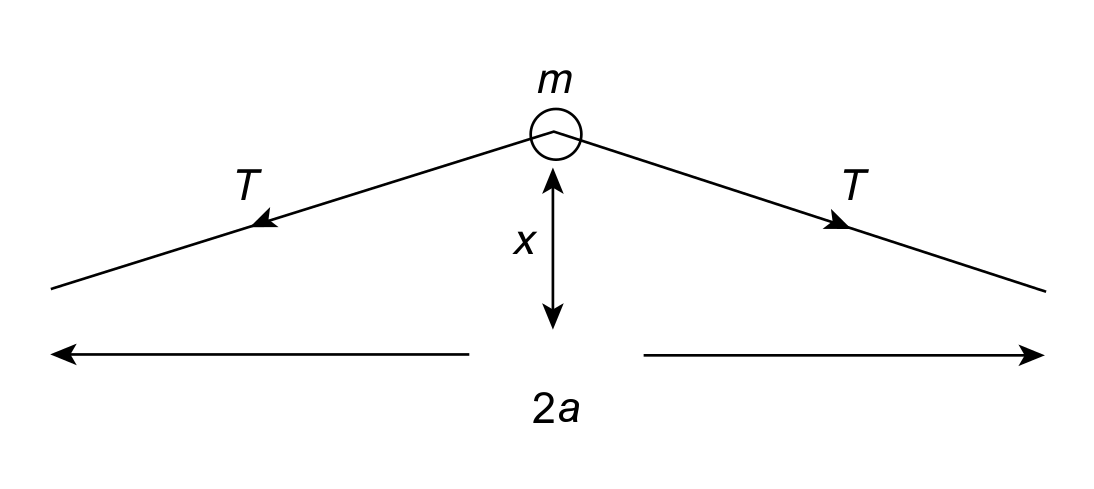
\includegraphics[width=0.5\textwidth]{Imagenes/transversal.png}
  \caption{Esquema del ejercicio de una masita moviendose transversalmente}
 \label{fig:masita_transversal}
\end{figure}

Consideramos, por el momento, sólo oscilaciones unidimensionales. En muchos casos tendremos sistemas que se puede considerar que tienen una dirección definida. En este caso, nos tenemos que imaginar que la ``dirección del sistema'' sería la de la recta que atraviesa todo el sistema cuando la masita está en el medio.

Una vez fijada esta dirección, vamos a distinguir, en relación a ella, dos tipos posibles de movimiento (que ni a palos serán los únicos) del integrante o los integrantes del sistema: \textbf{longitudinal} es un movimiento enteramente contenido en dicha dirección; \textbf{transversal} es un movimiento realizado exclusivamente en direcciones perpendiculares a la del sistema.

Ahora consideramos oscilaciones unidimensionales longitudinales de la masita. O sea, la masita está engarzada en un alambre recto (sin rozamiento) perpendicular a la dirección del sistema. Pongamos un sistema de referencia a lo largo de ese alambre, con $\psi=0$ cuando la masita está ``en el medio'' (los resortes, alineados). Para hallar la ecuación de movimiento hay que escribir adecuadamente la fuerza de cada resorte en función de $\psi$ y proyectarla adecuadamente en el sentido de movimiento.

La fuerza de cada resorte es $-k(l-l_0)$ en la dirección del resorte, pero $l$ depende de $\psi$. De hecho, a partir de un dibujo hecho para la masa en una posición $\psi$, a partir de un triángulo rectángulo sale $l = \sqrt{a^2+\psi^2}$ para cada resorte.

Para proyectar la fuerza en la dirección del alambre, consideramos momentáneamente el ángulo $\theta$ entre el resorte y el alambre. Entonces, para hacer la proyección basta multiplicar por $\cos{\theta}$; pero $\cos{\theta}=\frac{\psi}{l}$. Luego, la ecuación de movimiento resulta ser:
		\begin{align*}
			\ddot{\psi} &= -\frac{2k}{m}(l-l_0)\frac{\psi}{l} 
				= -\frac{2k}{m} \left(1-\frac{l_0}{l}\right) \psi\\
			\ddot{\psi} &= -\frac{2k}{m} \left(1-\frac{l_0}{\sqrt{a^2+\psi^2}}\right) \psi
		\end{align*}
Es una ecuación que no es lineal en $\psi$. No hay chance de resolverla sin restringirnos a la situación de \textit{pequeñas oscilaciones}.

Una advertencia: para hacer pequeñas oscilaciones alrededor de un punto de equilibrio (pensamos hacerlo en $\psi=0$, que en la ecuación de movimiento da $\ddot{\psi}=0$, como debe ser), debe asegurarse que sea de equilibrio estable. En esta situación, la estabilidad del equilibrio en $\psi=0$ excluye necesariamente que $a<l_0$. Uno podría llegar a imaginarse que si en la posición de equilibrio los resortes están comprimidos, cuando se corre un poquito la partícula los resortes intentarán seguir descomprimiéndose, para lo cual la alejarán más aun. Alternativamente, se puede calcular la derivada de $\ddot{\psi}$ \textit{respecto de $\psi$} y ver que para que la misma sea negativa en $\psi=0$ se debe tener $a\geq l_0$.

Para hacer pequeñas oscilaciones, hay que considerar $\psi$ muy chiquito, es decir, mucho menor que algún parámetro finito que intervenga en el problema. En este caso la comparación entra en juego en el radicando $a^2+\psi^2$; entonces pediremos que $|\psi| \ll a$. Una alternativa para trabajar consiste en tomar el término problemático no lineal $1-\frac{l_0}{\sqrt{a^2+\psi^2}}$ y hacerle un desarrollo en polinomio de Taylor (como función de $\psi$) alrededor de 0 hasta el segundo término no nulo.

Una forma más rápida involucra el siguiente truquito: si $|\psi| \ll a$ entonces $|\psi|/a \ll 1$ (y sus potencias naturales también), así que intentaremos ``intercalar'' un término así. Lo hacemos en la raíz:
		\[
			\frac{l_0}{\sqrt{a^2+\psi^2}}=\frac{l_0}{a\sqrt{1+(\psi/a)^2}} 
				= \frac{l_0}{a}\left[1+\left(\frac{\psi}{a}\right)^2\right]^{-1/2}
		\]
y como $(\psi/a)^2 \ll 1$, usamos la famosa aproximación $(1+\epsilon)^\alpha \approx 1 + \alpha\epsilon$ para $|\epsilon| \ll 1$. Resulta:
		\[
			\frac{l_0}{\sqrt{a^2+\psi^2}} \approx \frac{l_0}{a}\left[1-\frac{1}{2}\left(\frac{\psi}{a}\right)^2\right]
		\]

El paso que queda es mezclar esto en la ecuación de movimiento, agrupar términos por potencias de $\psi$ y tirar todos los de orden superior al lineal:
		\begin{align*}
			\ddot{\psi} &= -\frac{2k}{m}\left[1-\frac{l_0}{a}\left(1-\frac{1}{2}\left(\frac{\psi}{a}\right)^2\right)\right] \psi \\
			\ddot{\psi} &= -\frac{2k}{m}\left[\left(1-\frac{l_0}{a}\right)+\frac{l_0}{2a^3}\psi^2\right] \psi
		\end{align*}
El segundo término del corchete dará lugar a un $\psi^3$, así que se tira. Finalmente:
		\begin{equation}
			\ddot{\psi} = -\frac{2k}{m}\left(1-\frac{l_0}{a}\right)\psi
                        \label{eq:oscilador_transversal_pequenias_oscilaciones}
		\end{equation}
que corresponde a un oscilador lineal con $\omega_0^2=\frac{2k}{m}(1-\frac{l_0}{a})$, con solución general ya conocida. NOtemos entonces que en el caso en el que podamos tomar la aproximaci\'on de resorte \textit{slinky} en el que $l_0 \ll a$ obtenemos que $\omega_{l}^2=\omega_{t}^2$ lo cual se le llama una \textit{degenraci\'on} y es consecuencia que ahora el sistema presenta una nueva simetr\'ia respecto a los ejes de oscilaci\'on. (Aclaraci\'on: Hacer el ejercicio de oscilaciones longitudinales para poder verificar lo dicho)


Se presenta un problema en el lamentable caso en que $l_0=a$: nuestra ecuación final da $\ddot{\psi}=0$ constantemente, lo cual no es una aproximación satisfactoria (¡$\psi$ debería ser una traslación, sería un equilibrio indiferente!). En ese caso, el término lineal es nulo y el de $\psi^3$ no lo es; ¡entonces este último no es despreciable! (Nada es despreciable frente a 0, salvo quizás 0). La forma correcta de hacer pequeñas oscilaciones en ese caso consiste en conservar ese término:
		\[
			\ddot{\psi} = -\frac{k}{ma^2}\psi^3,
		\]
ecuación que no es lineal y que no pretendemos resolver. Este es un ejemplo de situación que no admite aproximación lineal.

\paragraph{Oscilaciones verticales de un flotador} Si conocemos el teorema de Arquímedes (para el empuje de cuerpos sumergidos), podemos aprovecharlo para estudiar esta situación. Lo recordamos en una de sus versiones prácticas: si un cuerpo está (por lo menos parcialmente) sumergido en un fluido de densidad $\rho$, experimentará debido a éste una fuerza $E$, llamada \textit{empuje}, opuesta a la gravedad $g$ y de módulo:
		\[
			E=\rho g V_s,
		\]
		donde $V_s$ es el volumen de la parte del cuerpo que está sumergida. (Es común interpretar el factor $\rho V_s = m_d$ como la ``masa del líquido desalojado'' y por lo tanto a $E = m_d g$ como igual al ``peso del líquido desalojado'', dando lugar al enunciado más popular del teorema de Arquímedes).
		
Imaginemos un cuerpito cilíndrico que flota en la superficie del agua, un fluido de densidad $\rho$ como vemos en la figura \ref{fig:flotador}. Llamemos $m$ a su masa, $L$ a su extensión longitudinal y $S$ a su superficie transversal, y pongamos un sistema de referencias como el que se ve en la figura, con $y=0$ en la superficie libre. Supongamos, para que sea posible la flotación, que el cuerpo es menos denso que el agua ($m/(SL)=\rho$). 

\begin{figure}[H]
  \centering
  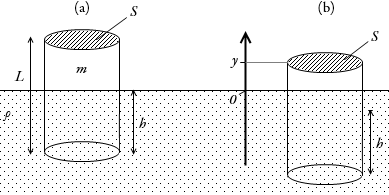
\includegraphics[width=0.5\textwidth]{Imagenes/flotador.png}
  \caption{Esquema del ejercicio de un cilindr flotando en un fluido}
 \label{fig:flotador}
\end{figure}

Ahora bien: si llamamos $y$ a la posición del extremo superior del cuerpo, resulta que $L-y$ es la longitud del cacho de cilindro que se encuentra sumergido, de modo que el volumen sumergido es $V_s = S(L-y)$ (siempre que $y<L$). Entonces, calculando el empuje e introduciéndolo (junto al peso) en la segunda ley de Newton resulta la ecuación de movimiento:
		\[
			m\ddot{y} = \rho g S (L-y) - mg
		\]
(En realidad el miembro de la derecha es $m\ddot{y}_\text{cm}$, pero hemos igualado $\ddot{y}=\ddot{y}_\text{cm}$ porque el cuerpito es rígido y no rota). Reordenando un poco:
		\[
			\ddot{y} = -\frac{\rho gS}{m} (y-L) - g =
				-\frac{\rho g S}{m}\left(y-L +\frac{m}{\rho S}\right)
		\]
La intricada artimaña aquí empleada tiene la finalidad de hacer ver que: (i) el punto $y= L-\frac{m}{\rho S}$ corresponde al equilibrio; (ii) el cambio de variable $\psi=y-L +\frac{m}{\rho S}$ convierte a la ecuación de movimiento en esta otra:
		\[
			\ddot{\psi} = -\frac{\rho g S}{m}\psi,
		\]
que es lineal y homogénea, y es la del oscilador armónico, con frecuencia $\omega_0^{\,2}=\frac{\rho g S}{m}$. Notar que llegamos a ella sin hacer uso de la aproximación por pequeñas oscilaciones: la solución es exacta (siempre que cumpla $y<L$; de lo contrario la ecuación de movimiento ¡tiene otra forma!).

Si nos interesa la variable original $y$, se la puede recuperar deshaciendo el cambio de variable. Una vez hallado $\psi$, se tendrá $y=\psi + L -\frac{m}{\rho S}$.

Observación: $\omega_0^{\,2}$ se puede escribir como $g/h$, con $h$ la profundidad del cuerpo sumergido en equilibrio.
		

\paragraph{Vibraciones ac\'usticas}

Consideremos una lampara con un volumen en el bulbo v y un tubo anexo de largo l y superficie lateral a como en la figura \ref{fig:bombilla}, a su vez supongamos que el volumen del tubo la es mucho menor que v. Entonces:\\

\begin{figure}[H]
  \centering
  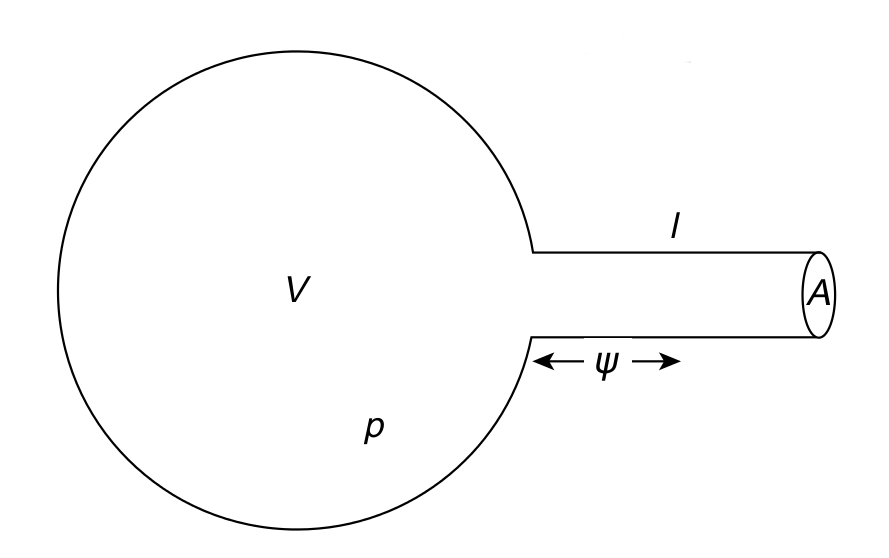
\includegraphics[width=0.5\textwidth]{Imagenes/bombilla.png}
  \caption{Esquema del sistema presentado para vibraciones ac\'usticas}
 \label{fig:bombilla}
\end{figure}

La masa del aire en el tubo es $la\rho$ y mediremos su desplazamiento \textit{hacia adentro} con la cantidad $ \psi$ . Llamemos a la diferencia neta de presi\'on $p$, entonces por la segunda ley de Newton tenemos:
\[(la\rho)\ddot{\psi}=-ap\]\\
Ahora hallemos la relacio\'on entre $\psi$ y $p$, que estar\'a dada por \textit{la compresibilidad} del aire:
\begin{equation}
\kappa=-\cfrac{1}{V}\left(\cfrac{\partial V}{\partial p}\right)
\label{compresibilidad}
\end{equation}
Para el aire en la lamparita el cambio de volumen es $\cfrac{a\psi}{v}$. Por lo que podemos decir\\
\[\kappa\approx \cfrac{a\psi}{vp}\]
Que lleva a:
\begin{equation}
\omega_0\approx\sqrt{\cfrac{a}{lv\rho\kappa}}
\end{equation}
\textbf{Observaci\'on}: Se obtuvo esa frecuencia usando la formula que se recuerda revisar, siempre vale posta!
\subparagraph*{Que compresibilidad??}
Antes de verificar num\'ericamente  la formula \ref{compresibilidad} tenemos que pensar que compresibilidad usamos, ya que el volumen \textbf{no} solo depende de la presi\'on sino que \textit{tambi\'en} de la temperatura. Primero debemos analizar \textit{que pasa} con la temperatura mientras sucede nuestro cambio de presi\'on. Una posibilidad es que no halla cambios en la temperatura, lo que nos llevar\'ia a usar la \textit{compresibilidad isot\'ermica} $\kappa_T$; que pasar\'ia si los cambios fuesen tan lentos que el flujo de calor es intercambiable a todo tiempo. \\
La otra posibilidad es que los cambios sean muy r\'apidos, llevando a una \textit{compresibilidad adiab\'atica} sin flujo de calor en si, $\kappa_S$. Claramente $\kappa_S \leq\kappa_T$ pues demanda mas presi\'on comprimir un gas si ademas se calienta. Finalmente le daremos la mano derecha a la compresi\'on adiab\'atica experimentalmente.
\subparagraph*{Evaluaci\'on num\'erica}
Suponiendo gases ideales, se tiene que $pV^\gamma=\mbox{cte}, \mbox{con} \ \gamma=\cfrac{C_p}{C_V}$ Por lo que por \ref{compresibilidad} tenemos $\kappa_S=\cfrac{1}{\gamma}p$.\\\\Por otro lado:
\[pV=RT \Longrightarrow \rho=\cfrac{M}{V}=\cfrac{Mp}{RT}\]
\[\Longrightarrow\ p\kappa_S=\cfrac{M}{\gamma}RT\]

\begin{equation}
	\omega_0 \approx \sqrt{{\left(\cfrac{a}{lv}\right)}{\left(\cfrac{\gamma R T}{M}\right)}}
\end{equation}

Es \'util notar que la frecuencia aumenta con $T^{1/2}$ pero es independiente de $p$. Esto ocurre porque tanto la masa como la "fuerza del resorte" que es inversamente proporcional a $\kappa_S$(que aqu\'i es el aire en el bulbo) son proporcionales a $p$. En general esperamos otras frecuencias un comportamiento parecido con otros factores geom\'etricos distintos a $\cfrac{a}{lv}$. Si insertamos valores obtenemos un $\omega_0 \approx 500 s^{-1}$ que se escucha como un grave \textit{plop}!

\paragraph{Vibraciones del Plasma}
 Un plasma es un gas con part\'iculas parcial o totalmente ionizadas, pero que se mantiene el\'ectricamente neutro. Para imaginarnos como puede vibrar simplemente basta con irradiar con luz UV un gas muy finamente durante un tiempo $t$. La luz UV al ser ionizante desacopla los electrones de las part\'iculas de gas obteni\'endose el plasma con $N$ iones positivos y electrones por unidad de volumen de plasma. Luego basta encender un campo el\'ectrico ortogonal a la proyecci\'on de la luz UV haciendo que tanto los electrones como los iones positivos se muevan ( como $m_p\gg m_e$ ignoraremos el movimiento de los iones positivos). Luego de un tiempo $t$ la capa de electrones se desplazo $\psi$ produciendo una capa negativa sin balancear de $-eN\psi$ por unidad de \'area. Aqu\'i ya basta con apagar el campo externo y hemos generado un campo interno:
\[E=\left(\cfrac{Ne}{\epsilon_o}\right)\psi\]\\
Que produce una fuerza el\'ectrica de retorno $F=-eE$ para cada electr\'on, llevando a la ecuaci\'on de movimiento para cada electr\'on:

\[\ddot{\psi} + \left(\cfrac{Ne^2}{m_e\epsilon_0}\right)\psi=0\]	
\\Llevando a una frecuencia
\begin{equation}
	\omega_0 = \sqrt{\cfrac{e^2}{m_e\epsilon_0}}.\sqrt{N}
	\label{frecuencia_plasma_simple}
\end{equation}

Podemos imaginar el conjunto de electrones como un fluido oscilante. Como casi todos los par\'ametros, excepto $N$ son constantes en \ref{frecuencia_plasma_simple} podemos tomar a la frecuencia de oscilaci\'on del plasma como una medida de la densidad electr\'onica en un plasma particular. Finalmente, para posteriores usos:
\begin{equation}
\cfrac{e^2}{m_e\epsilon_0}=3.18.10^3 \ m^3.s^{-2}
\label{constantes_plasma}
\end{equation}
Aunque parezca ficticio, este proceso sucede naturalmente y espont\'aneamente en la ionosfera, capa de la atm\'osfera a unos $\approx 60$ km. All\'i podemos identificar dos capas distintivas, la mas baja (la D)  con un $N \approx 10^9 \ m^{-3}$ al mediod\'ia. Por otro lado la capa mas alta (la capa $F_2$) toma valores de $N \approx 10^{12} \ m^{-3}$, entonces con la ayuda de\ref{frecuencia_plasma_simple} y \ref{constantes_plasma} podemos obtener frecuencias $\omega_0 \approx 2.10^6 \ s^{-1}$ ($v_o \approx 300 \ kHz$) para la capa D y de $\omega_0 \approx 6.10^7 \ s^{-1}$ ($v_o \approx 10 \ MHz$) para la capa $F_2$. Estas frecuencias son t\'ipicamente de radio y luego veremos que es lo que ayuda a las ondas de radio cortas poder reflejarse en la capa $F_2$ y entonces poder transmitirse a zonas lejanas a pesar de la curvatura de la Tierra.  

\section{Movimiento arm\'onico simple amortiguado}

En general nuestro modo de analizar las oscilaciones hasta ahora era bastante \textit{naive} considerando que la energ\'ia se conservaba siempre y no exist\'ian fuerzas disipativas, ahora vamos a complicar un poco m\'as el modelo y vamos a poder explicar mucho m\'as sucesos...

\subsection{El modelo}

Tomamos un oscilador arm\'onico de los de antes, y lo sumergimos en fluido en reposo. Debido a la viscosidad del fluido, aparecer\'a sobre el cuerpo una fuerza \textbf{retardadora}, opuesta a la velocidad relativa del cuerpo, y que \textit{en primera aproximaci\'on} sea proporcional a la misma. Llamando $\psi$ al desplazamiento del cuerpo respecto del equilibrio, debido al rozamiento viscoso aparece una fuerza de la pinta $-b\dot{\psi}$, con $b>0$ una constante, que da lugar, en la ecuaci\'on de movimiento, a un t\'ermino que va como $-\gamma \dot{\psi}$, con $\gamma=b/m$.

La ecuaci\'on de movimiento resulta ser:
		\begin{equation}
			\ddot{\psi} = - \omega_0^{\,2} \psi - \gamma \dot{\psi}
                        \label{eq:oscilador_amortiguado}
		\end{equation}
que, como es lineal, podemos intentar resolver hallando una base de soluciones proponiendo, como antes:
		\[\psi(t) = e^{\lambda t}.\]
		
Al reemplazar $\psi$ y sus derivadas en la ecuaci\'on de movimiento para hallar los posibles $\lambda$ se obtiene
		\begin{align*}
			&\lambda^2 e^{\lambda t} + \gamma\lambda e^{\lambda t} + \omega_0^{\,2} e^{\lambda t} = 0
			& & \text{pero }e^{\lambda t} \neq 0:\\
			&\lambda^2 + \gamma\lambda + \omega_0^{\,2}=0
		\end{align*}
La expresi\'on del miembro izquierdo se llama \textit{polinomio caracter\'istico} (en la variable $\lambda$) de la ecuaci\'on diferencial. Los $\lambda\in\C$ que sirvan deber\'an ser ra\'ices de ese polinomio. Como es de grado 2, se pueden hallar con la f\'ormula:
		\begin{equation}
			\lambda = -\frac{\gamma}{2} \pm \beta = -\frac{\gamma}{2} \pm \sqrt{\left(\frac{\gamma}{2}\right)^2 - \omega_0^{\,2}}
                      \label{eq:oscilador_amortiguado_raices}
		\end{equation}
El comportamiento de la soluci\'on, cuando tomemos parte real, depender\'a de que $\lambda$ sea real o no, lo cual depende directamente del signo de $\beta^2 = (\gamma/2)^2 - \omega_0^{2}$. 

Entonces, seg\'un los par\'ametros del sistema (¡y nunca las condiciones iniciales!), se distinguen tres tipos de soluciones. Si $\gamma/2<\omega_0$, se dice que el movimiento ser\'a \textit{subamortiguado}; si $\gamma/2>\omega_0$, se llama \textit{sobreamortiguado}; y si $\gamma/2=\omega_0$, se llama \textit{cr\'iticamente amortiguado} o se dice que hay \textit{amortiguamiento cr\'itico}.
		
%Podemos agregarle al oscilador arm\'onico una fuerza dependiente de la velocidad, que hace que la energ\'ia del sistema se disipe y se amortigue el movimiento. Es decir, la forma funcional general del oscilador arm\'onico amortiguado es
%    \begin{equation}
%        \ddot{\psi} = - \omega_0^2 \psi - \gamma \dot{\psi}
%        \label{eq:oscilador_amortiguado}
%    \end{equation}
    
%Que suponiendo una soluci\'on del estilo $\psi=A.\exp{\lambda t}$ nos da la ecuaci\'on algebraica caracter\'istica 
%\[\lambda^2 + \gamma \lambda + \omega_0^2 = 0\]
%Con dos ra\'ices a saber:
%\begin{equation}
%\lambda = -\cfrac{1}{2}\gamma \pm \sqrt{\cfrac{\gamma^2}{4}- \omega_0 ^2}
%\label{raices_caracteristica_amortiguado}
%\end{equation}
 
%Como vemos el tipo de soluciones de nuestro sistema depender\'a de los par\'ametros! 
%Llamaremos soluci\'on \textit{subamortiguada} cuando $\gamma < 2\omega_0$, soluci\'on \textit{sobreamortiguada} cuando $\gamma > 2\omega_0$, y soluci\'on \textit{cr\'iticamente amortiguada} cuando $\gamma = 2\omega_0$.

\paragraph{Movimiento subamortiguado}

Para el caso $\gamma/2<\omega_0$, $\beta^2<0$; entonces $\beta$ es imaginario puro:
		\begin{align*}
			\beta^2 =\left(\frac{\gamma}{2}\right)^2-\omega_0^{\,2}
			\qquad \Rightarrow \qquad
			\beta   =\pm i \sqrt{\omega_0^{\,2} - \left(\frac{\gamma}{2}\right)^2} = \pm i\omega,
		\end{align*}
donde llamamos $\omega = \sqrt{\omega_0^{\,2} - \left(\frac{\gamma}{2}\right)^2}$. Así,
		\begin{align*}
			&\lambda = -\frac{\gamma}{2} \pm i \omega.
		\end{align*}
Entonces, una soluci\'on (compleja) debe ser de la forma
		\begin{equation}
			\psi(t) = e^{(-\frac{\gamma}{2} + i \omega)t} = e^{-\frac{\gamma}{2}t} e^{i\omega t}.
                        \label{eq:oscilador_amortiguado_subamortiguado}
		\end{equation}
Tomando parte real y parte imaginaria obtenemos dos soluciones:
		\begin{align*}
			\psi(t) = e^{-\frac{\gamma}{2}t}\cos{\omega t}, &\psi(t)	= e^{-\frac{\gamma}{2}t}\sen{\omega t}
		\end{align*}
que, como son base, permiten expresar la soluci\'on general:
		\begin{align*}
			\psi(t) &= Ae^{-\frac{\gamma}{2}t}\cos{\omega t} + Be^{-\frac{\gamma}{2}t}\sen{\omega t}\\
				&= e^{-\frac{\gamma}{2}t} (A \cos{\omega t} + B \sen{\omega t})\\
				&= e^{-\frac{\gamma}{2}t} (\tilde{A} \cos{(\omega t + \phi_0)}),
		\end{align*}

con $\tilde{A}, \phi_0$ dependientes de las condiciones iniciales. La soluci\'on se trata de una oscilaci\'on arm\'onica, ``apantallada'' por el factor $e^{-\frac{\gamma}{2}t}$ que tiende a 0 cuando $t\to+\infty$. Interpretando $\tilde{A}e^{-\frac{\gamma}{2}t}$ como una ``amplitud variable'', se puede decir que esta soluci\'on es una oscilaci\'on arm\'onica con amplitud decreciente en el tiempo. Notar que la frecuencia $\omega$ de esta oscilaci\'on es distinta de la del oscilador ``libre'' $\omega_0$, por la presencia del t\'ermino $\gamma/2$.
		
%Aqu\'i tendremos soluciones complejas a la ecuaci\'on \ref{raices_caracteristica_amortiguado} con lo que escribiremos 
	
%	\[ \lambda = -\cfrac{1}{2}\gamma \pm i\omega_f\]
	
%Con 

	
%	\[\omega_f\equiv\sqrt{\omega_0 ^2 - \cfrac{\gamma ^2}{4}}= \omega_0\sqrt{1-\left(\cfrac{\gamma}{2\omega_0}\right)^2}\]
	

%Lo que nos lleva a unas soluciones del estilo

 %   \begin{equation}
%        \psi(t) = A e^{-\cfrac{\gamma}{2} t} e^{i (\omega_f t + \phi_0)},
%        \label{eq:oscilador_amortiguado_sub_solucion}
%    \end{equation}
    
\paragraph{Decaimiento de la energ\'ia}

La fuerza retardadora que incorporamos es de car\'acter \textit{disipativo}, pues al ser siempre contraria a la velocidad, lo es al desplazamiento, de manera que siempre realiza trabajo negativo; es decir, se pierde energ\'ia mec\'anica $E$, es disipada por la fuerza. Para conocer su evoluci\'on se puede calcular el trabajo $W$ de la fuerza disipativa entre el instante 0 y cualquier momento $t$:
                \begin{equation}
			E(t) - E(0) = W = \int_0^{t} F(t)\dot{\psi}(t) \,dt,
		\end{equation}
donde $F(t) = -m\gamma\dot{\psi}$ es la fuerza disipativa y el integrando $F(t)\dot{\psi}(t)$ es la potencia. Podr\'ia calcularse $E(0)$, hallar $\dot{\psi}$ y evaluar la integral. Pero un camino m\'as directo sale de la expresi\'on de $E$ como suma de la energ\'ia cin\'etica y el potencial:
		\begin{equation}
			E = T + V = \frac{1}{2}(m\dot{\psi}^2+k\psi^2)
				= \frac{1}{2}m(\dot{\psi}^2+\omega_0^{\,2}\psi^2)
		\end{equation}

Ahora bien,
		\begin{align*}
			\psi(t) & = A e^{-\frac{\gamma}{2}t} \cos{(\omega t + \phi_0)}\\
			\psi(t)^2 & = A^2 e^{-\gamma t} \cos^2{(\omega t + \phi_0)};\\
			\dot{\psi}(t) &= A e^{-\frac{\gamma}{2}t} ( -(\gamma/2) \cos{(\omega t + \phi_0)}
				- \omega \sen{(\omega t + \phi_0)} )\\
				&= -A e^{-\frac{\gamma}{2}t} \sqrt{(\gamma/2)^2+\omega^2} \cos{(\omega t + \phi_0 + \theta)}\\
				&= -A e^{-\frac{\gamma}{2}t} \omega_0 \cos{(\omega t + \phi_0 + \theta)}\\
			\dot{\psi}(t)^2 &= A^2 e^{-\gamma t} \omega_0^{\,2} \cos^2{(\omega t + \phi_0 + \theta)},
		\end{align*}
donde usamos que $-(\gamma/2) \cos{(\omega t + \phi_0)} - \omega \sen{(\omega t + \phi_0)}$ puede expresarse como un \'unico t\'ermino oscilante con amplitud $\sqrt{(\gamma/2)^2+\omega^2}=\omega_0$ y desfasaje $\theta$.

Reemplazando en $E$ y tomando factor com\'un resulta:
		\[
			E = \frac{1}{2}m A^2 \omega_0^{\,2} e^{-\gamma t} 
				(\cos^2{(\omega t + \phi_0)} + \cos^2{(\omega t + \phi_0 + \theta}))
		\]


% \paragraph{Energía media} En el laboratorio se suele trabajar con instrumentos que se basan en detectar la energía de un sistema. Supongamos que, en el intervalo que le lleva al instrumento detectar la energía, su valor oscila muchas veces alrededor de un cierto valor medio. En ese caso, lo que se observa generalmente es que la respuesta del instrumento corresponde, justamente, al valor medio de la energía $\vmed{H}$ en el intervalo de medición.

% Entonces, en situaciones donde se producen oscilaciones rápidas (o \textbf{ciclos rápidos}), resulta importante ver la evolución de las energías medias en cada intervalo.

% En las situaciones que consideremos, para simplificar los cálculos, intentaremos calcular valores medios de energía de manera de ``eliminar'' (o más bien absorber) la influencia del factor oscilante en la energía que se detecta, y en lo posible sin descuidar otros factores globales que afecten significativamente al sistema a lo largo de tiempos más largos (o más sensibles).

% En muchos casos será posible entender a la energía (u otras variables de interés) como un producto entre una función oscilante (llamada \textbf{portadora}) y otra función, llamada \textbf{moduladora}, de manera que la oscilación de la portadora (su frecuencia) es suficientemente rápida como para despreciar el cambio en la moduladora en un ciclo individual.

% Cuando la presencia de los factores disipativos sea débil ($\gamma \ll \omega$), será cierto que el factor de decaimiento exponencial se mantenga aproximadamente constante en un ciclo rápido: ya sea porque la oscilación es suficientemente rápida, o porque el amortiguamento es suficientemente suave.

% La duración o \textit{período} de un ciclo rápido viene dado, en función de la frecuencia, por $T=\frac{2\pi}{\omega}$. La energía media $\vmed{H}$ en el intervalo que dura un ciclo que comienza en el instante $t$, $[t; t+T]$, se calcula, por definición, como:
% 		\[
% 			\left.\vmed{H}\right|_t^{t+T}=\frac{1}{T}\int_t^{t+T}H(t')\, dt'
% 		\]
% Fijada la longitud del intervalo de integración (el período del ciclo rápido), convenimos en escribir a esta cantidad (que es función del instante $t$ representativo del ciclo):
% 		\[
% 			\vmed{H(t)}_{T}=\frac{1}{T}\int_t^{t+T}H(t')\, dt'
% 		\]
% Ahora bien: el factor modulador, que es aproximadamente constante en el intervalo, puede ser aproximado con muy poco error por su valor en el instante $t$ y sacado fuera de la integral. En el integrando queda sólo el factor de oscilación rápida. Si tiene período $T$, entonces la integral vale lo mismo que si se la evalúa en el intervalo $[0; T]$ (o cualquier otro intervalo de longitud $T$, para el caso).

% es posible entender a la energía como un producto entre una función oscilante y otra función, llamada habitualmente \textbf{moduladora}. La oscilación es ``rápida'', queriendo decir esto que la frecuencia es tan grande que, en el transcurso de una oscilación (o \textbf{ciclo}), la función moduladora se mantiene \textit{aproximadamente constante}. 



% Por otro lado, como la energía es positiva, se puede considerar, en cada instante, el valor medio correspondiente al ciclo

Como podemos ver en \ref{eq:oscilador_amortiguado} la fuerza de resistencia siempre se opone al movimiento, constantemente quitando energ\'ia a nuestro oscilador. ¡Veamos esto! Similarmente a lo hecho en \ref{energia_oscilador_derivada} llegamos a que 

\[\dot{E}=\dot{\psi}\left(m\ddot{\psi}+s\psi\right)\]

Y entonces por \ref{eq:oscilador_amortiguado} tenemos

\begin{equation}
  \dot{E}=-b\dot{\psi}^2\leq0\ \forall{t} \in \R 
\end{equation}

Lo que nos muestra de manera muy clara como siempre se va perdiendo energ\'ia, dependiendo linealmente del factor amortiguante!\\
La ecuaci\'on anterior es valida para todos los tipos de amortiguamiento, en espec\'ifico para obtener $E(t)$ en el caso subamortiguado basta poner \ref{eq:oscilador_subamortiguado} en la expresi\'on de la energ\'ia. No obstante nos interesa mas el decaimiento de energ\'ia en un periodo completo de medici\'on, que se define como

\begin{equation}
\langle{E}\rangle \equiv \cfrac{1}{T} \int _{t=0} ^{t=T} E(t) dt
\label{promedio_temporal}
\end{equation}

Y en nuestro caso resulta ser

\begin{equation}
\langle{E}\rangle \approx \cfrac{1}{2} m {\omega_0}^2 A^2 e^{-\gamma t}
\end{equation} 

Lo que nos da a una perdida fraccional de energ\'ia

\begin{equation}
-\cfrac{1}{\langle{E}\rangle}.\cfrac{d\langle{E}\rangle}{dt} \approx \gamma
\label{perdida_proporcional_energia_oscilador}
\end{equation}

Punto donde empieza a ponerse interesante la definici\'on del gamma como factor del amortiguamiento.

\subparagraph*{Valor Q}
En vez de andar usando el valor $\cfrac{\gamma}{2\omega_0}$ para definir cuando hay amortiguamiento suave, es preferible definir un factor que cumpla nuestro requerimientos, al cual le llamaremos \textit{factor de calidad}:

\[Q\equiv\cfrac{\omega_0}{\gamma}\]

Por lo que podemos decir que nuestro sistema va a estar suavemente amortiguado cuando $Q>\cfrac{1}{2}$. Pr\'oximamente veremos nuevas ventajas de la definici\'on del factor de calidad.

\paragraph{Movimiento sobreamortiguado}
Si volvemos a \ref{eq:oscilador_amortiguado_raices} y ahora consideramos que $\gamma>2\omega_0$ obtenemos que las dos ra\'ices de la ecuaci\'on caracter\'istica son ambas reales y negativas! Como en general es mas c\'omodo trabajar con cantidades positivas definamos

\begin{equation*}
\mu_1\equiv -p_1=\cfrac{1}{2}\gamma + \sqrt{\left({\cfrac{\gamma^2}{4}-\omega_0^2}\right)} 
\end{equation*}

\begin{equation*}
\mu_2\equiv -p_2=\cfrac{1}{2}\gamma - \sqrt{\left({\cfrac{\gamma^2}{4}-\omega_0^2}\right)}
\end{equation*}

De lo que se ve que $\mu_1>\cfrac{\gamma}{2}>\omega_0$ tanto como $\mu_1\mu_2=\omega_0$ y entonces $\mu_2<\omega_0$. Obteniendo unas soluciones

    \begin{equation}
        \psi(t) = A e^{(-\mu_1 t)} + B e^{(-\mu_2 t)}
        \label{eq:oscilador_sobreamortiguado_soluciones}
    \end{equation}
 Aqu\'i podemos analizar un caso interesante que es el hecho que A y B \textbf{no necesariamente} son positivos! Cuando tenemos el hecho que (por las condiciones iniciales!) son de signo distinto, podemos llegar a tener que la masita pase \textit{una vez} la posici\'on de equilibrio y luego el movimiento muera, mientras que si son ambos positivos o negativos esto nunca ocurrira y nunca llegara a la posici\'on de equilibrio la masita; hecho y derecho este movimiento es \textit{aperi\'odico}.

\paragraph{Movimiento cr\'iticamente amortiguado}

 Finalmente cuando $\gamma=2\omega_0$ obtenemos una sola soluci\'on exponencial, que por cuesti\'on de independiencia lineal matem\'aticas terminamos teniendo estas soluciones
 
   \begin{equation}
        \psi(t) = (A + B t) e^{-\omega_0 t}
        \label{eq:oscilador_amortiguado_critico}
   \end{equation}
   
\textbf{Observaci\'on 1}: F\'isicamente podemos pensar en el caso subamortiguado, haciendo crecer el valor de $\gamma$ y pensar que las soluciones cumplen continuidad. En este caso podemos ver que al aumentar $\gamma$ la frecuencia $\omega_f$ se hace casi nula, perdiendo toda la curvatura y eso nos da una idea que la otra soluci\'on independiente debe ser una linea recta!
\textbf{Observaci\'on 2}: Matem\'aticamente podemos analizar el problema hallando la forma de Jordan de la matriz del sistema de ecuaciones diferenciales y de ah\'i se obtiene el termino lineal.    

Mucho mas no diremos aqu\'i salvo que notemos que el decaimiento es \textit{m\'aximo} en el caso cr\'iticamente amortiguado, dado que es linealmente exponencial.

Para terminar de cerrar la idea de este modelo, nada mejor que un gr\'afico, como el de la figura \ref{fig:oscilador_amortiguado} d\'onde tenemos los tres tipos de movimientos amortiguados para par\'ametros prefijados (cambiandolos simplemente cambias las escalas del tiempo y espacio). \textbf{Aclaración:} ahora es momento de ver todas los chirimbolos que definimos, y poder observar los patrones referidos

\begin{figure}[H]
  \centering
  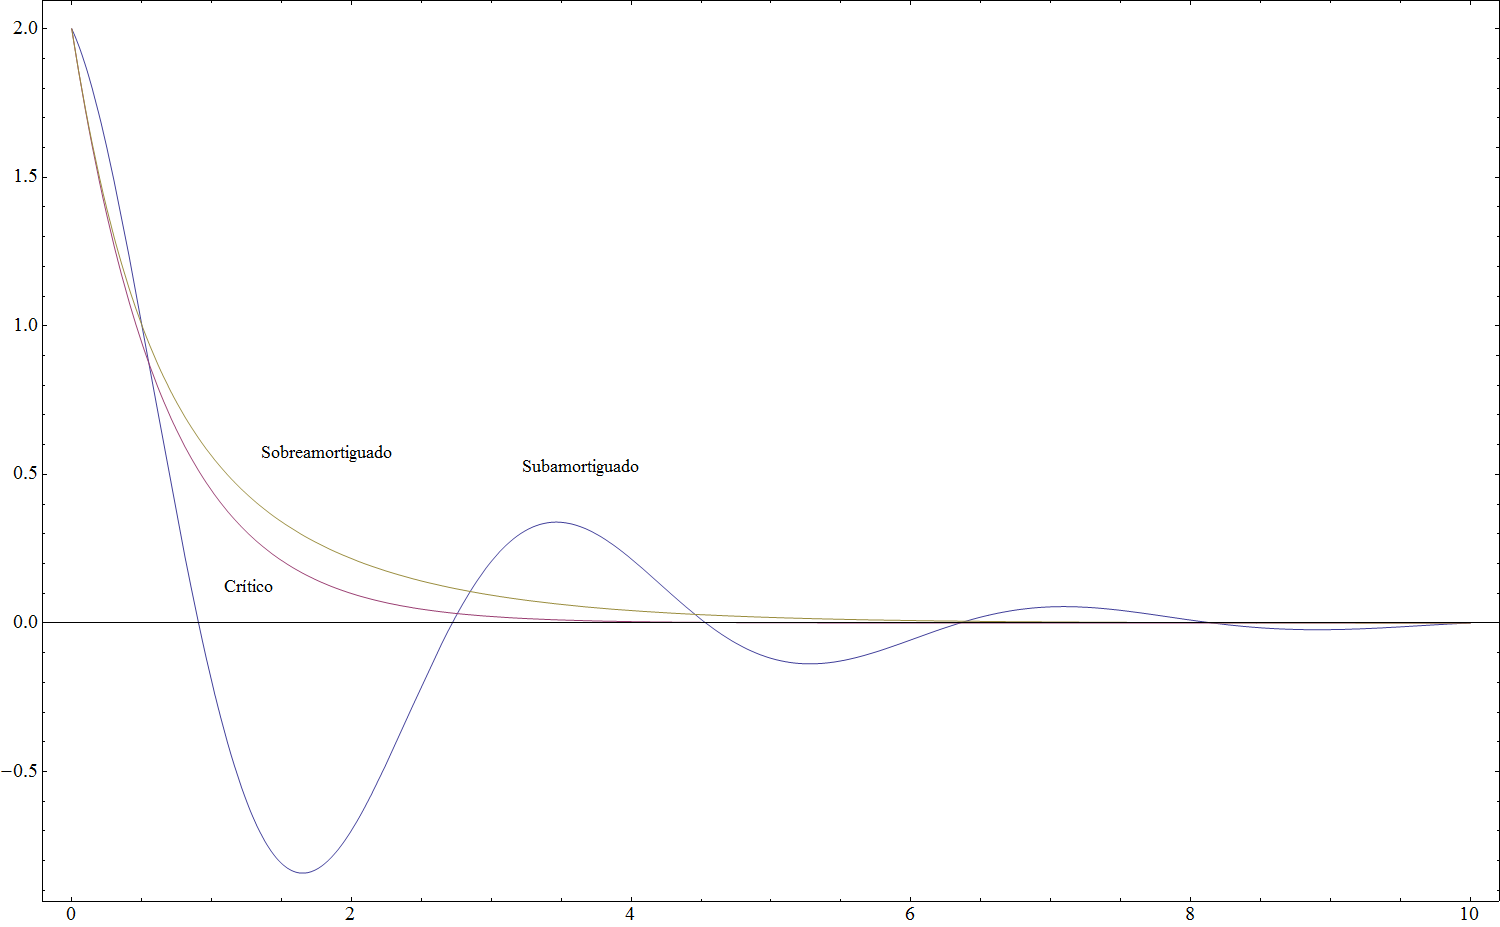
\includegraphics[width=0.8\textwidth]{Imagenes/amortiguado.png}
  \caption{Tres tipos de movimientos amortiguados}
  \label{fig:oscilador_amortiguado}
\end{figure}

\subsection{El movimiento amortiguado en la f\'isica}

An\'alogamente a lo anterior verificaremos algunos casos donde podemos modelar con un movimiento amortiguado simple de alg\'un tipo.	

\paragraph{Amortiguamiento por colisiones}
Volviendo a nuestro amigo el plasma visto antes, ah\'i pudimos ver que el origen del movimiento oscilatorio resultaba del comportamiento cooperativo de los electrones con una velocidad determinada $\dot{\psi}$. Sin embargo entonces no consideramos la \textit{agitaci\'on t\'ermica} que azarosamente produce una agitaci\'on que podr\'ia colisionar con los electrones contiguos, produciendo una dispersi\'on con direcci\'on al azar y , por ende, dejando de participar del grupo de electrones que aportan a la vibraci\'on en si. Esta \textit{p\'erdida} de electrones a la vibraci\'on del plasma debe ser proporcional a la densidad $N$ presente, y debe tener un tiempo car\'acter\'istico de decaimiento $\tau_c$. Podemos estimar:

\[-\cfrac{1}{N}\cfrac{dN}{dt}=\cfrac{1}{\tau_c}\]

Pero en contraparte a los otros tipos de amortiguamiento vistos, aqu\'i \textbf{no hay decaimiento en amplitud} sino en la densidad de electrones participantes. Por ende, en analog\'ia a \ref{perdida_proporcional_energia_oscilador} podemos estimar 

\[\gamma_c=\cfrac{1}{\tau_c}\]

\subparagraph*{Amortiguamiento en la ionosfera}
En la ionosfera los electrones son mas que proclives a colisionar con mol\'eculas neutras, y la tasa de colisiones debe ser proporcional a $N_m$ y a la velocidad de los electrones. La ultima esta dada por $v_{temp}$ que, vimos, supera a $\dot{\psi}$. Entonces:

\begin{equation}
\gamma_c=\sigma_c\left(N_mv_{temp}\right)
\end{equation}

Con $\sigma_c$ una constante de proporcionalidad, tiene unidades de \'area y puede pensarse como el \'area efectiva de choque dada por las mol\'eculas a los electrones; cuyo valor experimental ronda los $\sigma_c\approx 10^{-19} m^2$ El factor $N_m$ debe ser alto si hay una presi\'on alta y temperatura baja (son mol\'eculas neutras de la atm\'osfera), por ende suponiendo gases ideales:

\begin{equation}
N_m=\cfrac{p}{kT}
\end{equation} 

Con $k$ la constante de Bolztmann. Por otro lado suponiendo cada contribuci\'on cuadr\'atica aporta $\cfrac{1}{2}kT$, los electrones al tener 3 grados de libertad obtenemos

\[\cfrac{1}{2}m_e{v_{temp}}^2\approx \cfrac{3}{2}kT\]

Con lo que

\begin{equation}
v_{temp}\approx \sqrt{\cfrac{3kT}{m_e}}
\end{equation}

Juntando todo tenemos que 

\[\gamma_c\approx \sqrt{\cfrac{3\sigma_c ^2}{m_ek}}pT^{-\cfrac{1}{2}}\]

La presi\'on en la capa D de la ionosfera es de $p\approx0.5 N m^{-2}$ y la temperatura $T\approx 200 K$ con lo que tenemos $\gamma_c \approx 2.10^6 s^{-1}$ que si recordamos lo calculado previamente, son similares, por lo que las vibraciones del plasma en la capa D tienen un $Q\sim 1$.\\
En la capa $F_2$ por otro lado tenemos $p\approx 10^{-10} N m^{-2}$ y $T\approx 2000 K$ con lo cual, dado que ademas $\omega_{0F} \sim 10. \omega_{0D}$, tenemos que $Q \gg 1$ para la capa $F_2$ lo que resulta muy importante para las radiofrecuencias.

\paragraph{Amortiguamiento por fricci\'on}
Finalmente para terminar esta secci\'on nos pareci\'o importante analizar el caso del amortiguamiento por la fuerza de rozamiento usual que experimentamos por el contacto entre dos superficies dadas.

Si analizamos una masita, vemos que la ecuaci\'on de movimiento resulta ser

\[ m\ddot{\psi} = \left\{ \begin{array}{ll}
         -s\psi -F_d & \mbox{si $\dot{\psi}>0$};\\
         -s\psi +F_d & \mbox{si $\dot{\psi}<0$}.\end{array} \right. \] 

Que se parece mas a una ecuaci\'on libre que una amortiguada, dado que $F_d$ es invariante con respecto al modulo de $\dot{\psi}$. Una forma de desacoplar este sistema es proponiendo el cambio de coordenadas:

\begin{equation*}
\begin{array}{l}
\psi_d=\psi+\cfrac{F_d}{s} \\
\psi_i=\psi-\cfrac{F_d}{s}
\end{array}
\end{equation*}

Nos permite escribir

\begin{equation*}
\begin{array}{l}
\ddot{\psi_d}+\omega_0 ^2\psi_d=0 \\
\ddot{\psi_i}+\omega_0 ^2\psi_i=0
\end{array}
\end{equation*}

Para los movimientos a la derecha e izquierda respectivamente, y vemos ya est\'an plenamente desacoplados y el movimiento de la masita se compone de \textit{medio ciclos} yendo de $\psi_d$ a $\psi_i$ y viceversa, teniendo que, dada una amplitud inicial $A_1$ cada movimiento para en $A_1-2k\cfrac{F_d}{s} \qquad k \in \Z $ con la amplitud efectiva decayendo \textit{linealmente} con el numero de ciclos completados. Finalmente el movimiento se detendr\'a cuando al final de un \textit{medio ciclo} se obtenga que $m\ddot{\psi}<\vert{F_e}\vert$ con $F_e$ la fuerza de rozamiento est\'atico.

\section{Movimiento arm\'onico forzado}
Finalmente para completar nuestro estudio de las oscilaciones con un grado de libertad consideraremos el movimiento con posibilidad de aplicar fuerzas externas, que por motivos explicados luego al ver an\'alisis de Fourier, podemos suponer senoidal.

\subsection{El modelo}
Aqu\'i vamos a ampliar el modelo antes visto al agregarle una fuerza externa \textit{dependiente del tiempo} $F(t)$ que podemos considerar arm\'onica por motivos que veremos luego en el an\'alisis de Fourier:

\[ F(t)= F_0 \cos{\omega t} \]

Con esta fuerza nueva actuante la ecuaci\'on de movimiento se torna:

    \begin{equation}
        \ddot{\psi} + \omega_0 ^2 \psi + \gamma \dot{\psi} = F(t)
        \label{eq:oscilador_forzado}
    \end{equation}
    
Como sabemos de la teor\'ia de ecuaciones diferenciales toda soluci\'on $X(t)=X_h(t)+X_p(t)$ es la suma de la soluci\'on del sistema \textit{homog\'eneo} y una soluci\'on particular cualquiera. Si analizamos un poco el modelo notamos que ya tenemos la $X_h(t)=\psi(t)$ es la soluci\'on del sistema amortiguado, por ende nos basta averiguar la soluci\'on particular, para esto supongamos ya paso un tiempo $t\gg\cfrac{1}{\gamma}$, en este caso tenemos 
    
\[\lim_{t\rightarrow\infty} X_h(t)=0\]

Y por ende estaremos estudiando la soluci\'on particular al considerar el que llamamos el \textbf{estado estacionario} de la soluci\'on $X(t)$.

\paragraph{Estados estacionarios}

Intuitivamente sabemos que si la fuente externa pone la frecuencia de oscilaci\'on del sistema finalmente, pero que el sistema va a responder mejor si es parecida su frecuencia natural $\omega_0$. Proponiendo como soluci\'on particular $\psi = C e^{i \omega t}$ tenemos la intuici\'on que aunque el desplazamiento no necesariamente esta en fase con la fuerza, al menos la diferencia de fase \textbf{ya alcanzo un valor constante}. 

\subparagraph*{Enfoque 1}

Entonces obtenemos la siguiente ecuaci\'on\'on algebraica $(\omega_0^2 - \omega^2 + i \omega \gamma) C = \cfrac{F_0}{m}=A$, por lo que la amplitud es
	\begin{equation}
		C = \cfrac{A (\omega_0^2 - \omega^2 - i \omega \gamma)}{(\omega_0^2 - \omega^2)^2 + (\omega \gamma)^2} = \cfrac{A (\omega_0^2 - \omega^2)}{(\omega_0^2 - \omega^2)^2 + (\omega \gamma)^2} - i \cfrac{A \omega \gamma}{(\omega_0^2 - \omega^2)^2 + (\omega \gamma)^2}
		\label{eq:oscilador_forzado_particular_amplitud}
	\end{equation}
\\
\textbf{Recordatorio:} Para obtener la amplitud $C$ se uso la relaci\'on ya dispuesta que

\[\forall z\in\C^{*} \qquad z^{-1}=\cfrac{\overline{z}}{\vert{z}\vert}\]

Lo que nos da la soluci\'on

	\begin{equation}
		\psi_p(t) = \Rea \ (C) \cos(\omega t) + \Ima (C) \sen(\omega t) = C \cos(\omega t + \phi)
		\label{eq:oscilador_forzado_particular_soluci\'on}
	\end{equation}
	
que no tiene constante de integraci\'on ($\Rea \ $ es la parte real y $\Ima$ es la parte imaginaria) ya que dichas aparecen solamente en la soluci\'on homog\'enea. Ademas la soluci\'on homog\'enea decae por lo que luego de un tiempo (denominado transitorio) pasa a un estado estable o estacionario donde predomina la soluci\'on particular. La fase $\phi$ indica como esta desfasado el movimiento de la soluci\'on particular de la soluci\'on homog\'enea. Cabe notar que aqu\'i $\Ima{C}$ resulta que esta en cuadratura con la fuerza $F(t)$  y $\Rea \ (C)$ esta en fase con la fuerza, es costumbre notar a la componente en cuadratura como $A_{abs}$ (de amplitud absorbente)y a la componente en fase como $A_{el}$ (de amplitud el\'astica). Con lo que queda

\begin{equation}
\psi_{p} (t)= A_{abs}\sin(\omega t)+A_{el}\cos(\omega t)
\label{solucion_particular_forzado}
\end{equation}

Donde la componente absortiva se vuelve m\'axima en las frecuencias cercanas a la natural del sistema (despu\'es veremos que tan cercanas) y la el\'astica es pr\'acticamente nula; y viceversa fuera de la zona de $\omega_0$. Esto nos lleva a decir que la componente absortiva es la dominante en la zona de $\omega \sim \omega_0$ y la el\'astica fuera de ella. El otro factor notorio es que $A_el$ cambia el signo al pasar $\omega_0$ y esto representa un cambio en el modo de vibraci\'on del sistema que luego se volver\'a mas frecuente analizar (con 1 masa lo remarcamos y no le veremos mucho significado f\'isico ya que la amplitud decae fuera de $\omega_0$).

Para simplificar la notaci\'on uno suele definir la \textbf{impedancia mec\'anica} de un sistema como

\begin{equation}
Z=m\left(\gamma\omega+i\left(\cfrac{\omega^2 - \omega_0 ^2}{\omega}\right)\right)
\label{definicion_impedancia}
\end{equation}

Donde a la parte real le llamamos \textbf{resistencia} y a la imaginaria \textbf{reactancia}. Con lo cual en \ref{eq:oscilador_forzado_particular_amplitud} nos queda

\[C=\cfrac{-iA}{Z}\]

Entonces observemos que $C=\cfrac{\dot{\psi}}{i\omega}$ con lo que tenemos

\[F(t)= m\left((\omega_0^2 - \omega^2 + i \omega \gamma)\right)\cfrac{\dot{\psi}}{i\omega}\]
\textbf{Recordatorio}: Lo anterior provino de la ecuaci\'on car\'acter\'istica del sistema forzado

Con lo que reagrupando conseguimos la siguiente relaci\'on que justifica la definici\'on de impedancia:

\begin{equation}
F=Z\dot{\psi}
\end{equation}

\textbf{Con lo que la impedancia mec\'anica es la fuerza necesaria para producir velocidad unitaria en un oscilador!!}

\subparagraph*{Enfoque 2}

El segundo enfoque posible para obtener la amplitud de la soluci\'on particular $\psi_p$ consiste en el uso de fasores o Diagramas de Argand (Jean Robert Argand (1768 -1822) matem\'atica talentoso que introdujo el concepto de representar a los n\'umeros complejos como punto de un $\R$ espacio vectorial isomorfo a $\R^2$). Para esto uno representa el modulo de su numero complejo y con el angulo $\phi$ representa el desfasaje del pr\'oximo numero respecto al primero, pero dado que estamos en un estado estacionario donde la diferencia de fase $\varphi=cte$ podemos diagramar a $t=0$ y todo el diagrama conjunto rotara $\forall t$ haciendo valido nuestro calculo de las sumas iniciales.

%ACA PONER EL GRAFICO DE FASORES%
\begin{figure}[H]
  \centering
  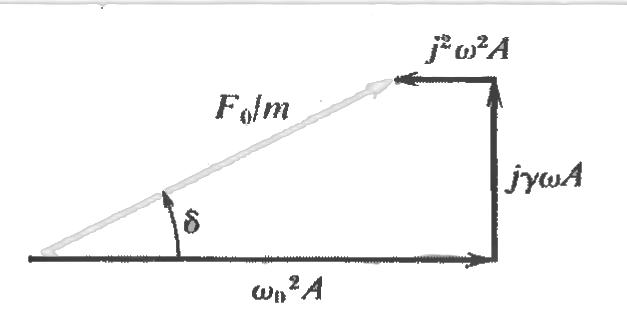
\includegraphics[width=0.5\textwidth]{Imagenes/fasores.png}
  \caption{Representación fasorial de la ecuación del oscilador forzado}
  \label{fig:oscilador_forzado_fasores}
\end{figure}

Del gr\'afico \ref{fig:oscilador_forzado_fasores} (llamando $j = i$, la unidad imaginaria, y a $\delta = -\phi$, la fase) f\'acilmente se ve que primero que $-\pi<\phi<0$ por lo que \textit{el desplazamiento siempre esta retrasado a la fuerza impulsora en $\phi$}. Por otro lado viendo el triangulo rect\'angulo dado se ve:

\begin{equation}
\tan{\phi}=\cfrac{-\gamma\omega}{\omega_0 ^2 - \omega^2}
\label{fase_forzado_variacion}
\end{equation}

Que notemos no contiene en ning\'un lado a $F_0$ por lo que la diferencia de fase \textbf{solo depende de la frecuencia impulsora}. Por otro lado aplicando pit\'agoras obtenemos

\[A^2=C^2\left(\left(\omega_0 ^2 - \omega^2\right)^2 + \gamma^2\omega^2\right)\]

De donde obtenemos

\begin{equation}
C=A\sqrt{\cfrac{1}{\left(\omega_0 ^2 - \omega^2\right)^2 + \gamma^2\omega^2}}
\end{equation}

Para simplificarnos la vida podemos utilizar la que se llama \textit{curva de respuesta}:

\begin{equation}
R(\omega)=\cfrac{\gamma^2\omega^2}{\left(\omega_0 ^2 - \omega^2\right)^2 + \gamma^2\omega^2}
\end{equation}

Que, si notamos, para un sistema muy poco amortiguado $Q \ll \cfrac{1}{2} \qquad \omega \sim \omega_0$ se puede aproximar muy bien por la curva que llamamos \textit{Lorentziana} que se define como

\begin{equation}
L(\omega)= \cfrac{\cfrac{\gamma^2}{4}}{\left(\omega_0 ^2 - \omega^2\right)+\cfrac{\gamma^2}{4}}
\label{Lorenztiana}
\end{equation}

Con lo cual tenemos para, respectivamente, las amplitudes de la posici\'on, velocidad y aceleraci\'on:

\begin{equation}
\begin{array}{rcl}
A & = & \left(\cfrac{F_0}{b\omega}\right)\sqrt{R(\omega)} \\
A\omega & = & \left(\cfrac{F_0}{b}\right)\sqrt{R(\omega)} \\
A\omega^2 & = & \left(\cfrac{F_0\omega}{b}\right)\sqrt{R(\omega)} 
\end{array}
\label{curvas_respuestas_forzado}
\end{equation}
\\
Con lo que se ve que la velocidad alcanza su m\'aximo en $\omega=\omega_0$ pero la posici\'on lo alcanza a un valor un poco menor y la aceleraci\'on a un valor un poco mayor, como se puede ver en la figura \ref{fig:oscilador_forzado_respuesta}. (los valores se pueden hallar derivando, etc, etc...). A su vez vemos que para $\omega<\omega_0 \ \cfrac{F_0}{k}\leq \psi$ y para $\omega>\omega_0 \ \cfrac{F_0}{m}\leq \ddot{\psi}$. Que esta bueno analizar y se lo dejamos al lector! (sino tiene todo servido che!)

\begin{figure}[H]
  \centering
  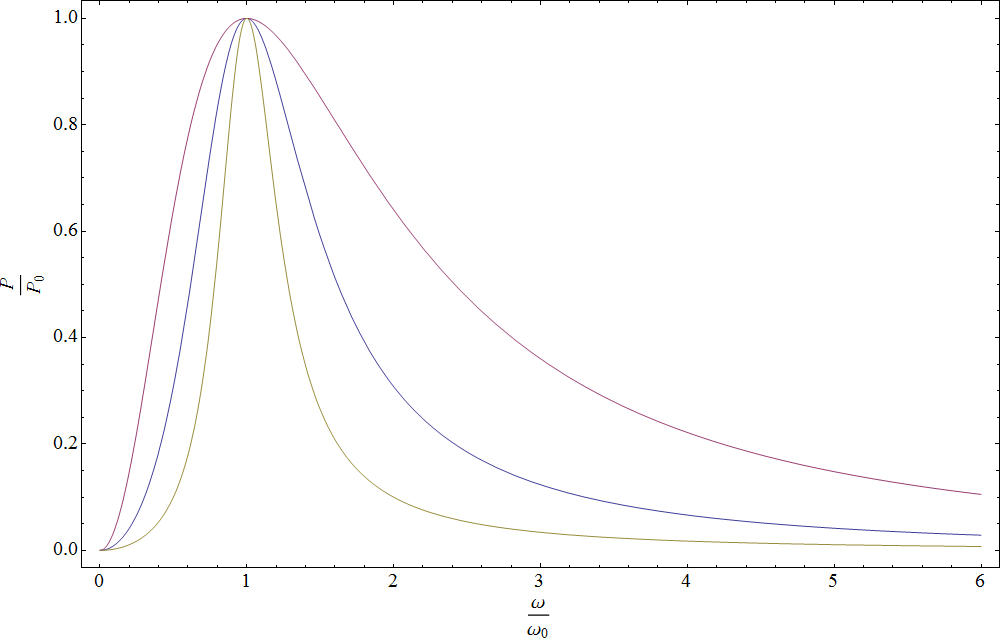
\includegraphics[width=0.5\textwidth]{Imagenes/resonancia.png}
  \caption{Respuesta en frecuencia de un oscilador forzado, para la velocidad, para diferentes valores de $Q$}
  \label{fig:oscilador_forzado_respuesta}
\end{figure}

Y ahora decimos listo, pero para y la impedancia? y buen vamos a ver que onda con este nuevo enfoque en que nos puede aportar algo nuevo (para lo viejo ya vimos todo lo otro).

Tal como definimos la funci\'on \textit{real} de respuesta $R(\omega)$ vamos a definir otra funci\'on nueva de respuesta llamada \textit{compliancia} (\textbf{Aclaracion:} cualquier mejor traducci\'on del ingles \textit{compliance} es bienvenida).
Dada una $\psi (t) = A e^{i\omega t}\qquad A\in\C$

\begin{equation}
K(\omega)=\cfrac{A}{F_0}
\end{equation}

Entonces volviendo al diagrama podemos ver

\begin{equation*}
\begin{array}{rcl}
\cos{\phi} & = & \cfrac{mA\left(\omega_o ^2 - \omega^2\right)}{F_0} \\
\sin{\phi} & = & \cfrac{mA\gamma\omega}{F_0}
\end{array}
\end{equation*}

De lo que obtenemos

\begin{equation}
\begin{array}{rcccl}
\Rea \ {K(\omega)} & = & \cfrac{A\cos{\phi}}{F_0} & = & \cfrac{\omega_0 ^2 - \omega^2}{\left(\omega_0 ^2 - \omega^2\right)^2 + \gamma^2\omega^2} \\
\Ima{K(\omega)} & = & \cfrac{A\sin{\phi}}{F_0} & = & \cfrac{\gamma\omega}{\left(\omega_0 ^2 - \omega^2\right)^2 + \gamma^2\omega^2} 
\end{array}
\end{equation}

Y aunque se ve medio fea $K(\omega)$ la podemos hacer linda con un poquiiito de cuentas y nos termina dando

\begin{equation}
K(\omega)=\cfrac{1}{\left( k-m\omega^2\right) + ib\omega}
\end{equation}

Y aunque nos guste trabajar ne reales admitamos que trabajar con complejos puede ser mucho mas simple, ya que todos los denominadores al cuadrados al ser en general m\'odulos nos los sacamos de encima! Finalmente recordando \ref{definicion_impedancia} tenemos que

\begin{equation}
Z(\omega)=\cfrac{1}{i \omega K(\omega)}=b + i\left(m\omega-\cfrac{k}{\omega}\right)
\end{equation}

Y entonces veamos que $Z(\omega_0)=b \ \in\R$ con lo cual en general es muy com\'un para hallar la frecuencia natural de un sistema, hallar $\omega \in \R \ / \ Z(\omega)\in\R$. Lo importante es que \textbf{una impedancia real implica que la velocidad esta en fase con la fuerza impulsora}.

Ahora que analizamos ambos enfoques, ya podemos asegurar conseguimos la soluci\'on $\psi_p$ (se acuuuerdan eso quer\'iamos nosotros?) y podemos analizar como varia la soluci\'on en los diferentes casos que llamaremos \textit{amortiguamiento suave} cuando $Q>\cfrac{1}{2}$ y \textit{amortiguamiento fuerte} cuando $Q \ll \cfrac{1}{2}$

\paragraph*{Amortiguamiento suave}

Recordemos \ref{curvas_respuestas_forzado} de donde podemos ver un efecto importante, cerca de $\omega_0$ todas las amplitudes resultan significativas, y la fase cambia dr\'asticamente (notar de \ref{fase_forzado_variacion} como varia de 0 a $-\pi$ en la zona que llamaremos \textit{de resonancia}. De la fase podemos destacar que en $\omega=\omega_0 \qquad \phi=-\cfrac{\pi}{2}$ por lo que el desplazamiento retrasa a la fuerza en cuadratura y entonces, como hab\'iamos visto antes, \textbf{en la resonancia la velocidad esta en fase con la fuerza y la impedancia resulta real}.
Si consideramos el caso de frecuencias muy bajas ($\omega\ll\omega_0$) tenemos

\begin{equation}
\begin{array}{rcccl}
\phi & \approx & 0 \\
A & \approx & \cfrac{F_0}{m\omega_0 ^2}&=& \cfrac{F_0}{k} \\
\psi & \approx & \left(\cfrac{F_0}{k}\right) \cos{\omega t}
\end{array}
\label{aproximacion_frecuencias_bajas_forzado}
\end{equation}

Notemos que ni $m$ ni $\gamma$ esta involucrados ac\'a lo que nos lleva a decir que a frecuencias bajas el movimiento se encuentra \textit{controlado por el resorte}, y es f\'acil de entender. La masa tiene muy poca aceleraci\'on haciendo que la mayor\'ia de la fuerza impulsora se contrarreste con la fuerza de retorno del resorte, provocando entonces que el desplazamiento este en fase con la fuerza, como \ref{aproximacion_frecuencias_bajas_forzado} verifica. Por otro lado a altas frecuencias ($\omega\gg\omega_0$) tenemos

\begin{equation}
\begin{array}{rcl}
\phi & \approx & -\pi \\
A & \approx & \cfrac{F_0}{m\omega^2}\\
\psi & \approx & \left(\cfrac{F_0}{m \omega^2}\right) \cos{\omega t}
\end{array}
\label{aproximacion_frecuencias_altas_forzado}
\end{equation}

Y decimos que el movimiento es \textit{controlado por la masa} donde el resorte b\'asicamente no hace nada y todo lo hace la fuerza impulsora, por lo que los resultados de \ref{aproximacion_frecuencias_altas_forzado} es de esperar.

Lo ultimo a notar es que 

\[\lim_{{\gamma \rightarrow 0}\atop{\omega \rightarrow \omega_0}} A \left(\omega\right) = \infty \]

Por lo que decimos el movimiento en $\omega \sim \omega_0$ es \textit{limitado por la resistencia} (Como el imperio gal\'actico =P)

La resonancia provee amplificaci\'on, una redistribuci\'on de la vibraci\'on podr\'iamos decir, y en que factor sino en $Q$, que nos daba la suavidad del amortiguamiento $Q\equiv \cfrac{\gamma}{\omega_0}$

\paragraph{Energ\'ia y Potencia}
Como nos podemos imaginar para todo tiempo el amortiguamiento esta sacando energ\'ia de nuestro sistema, lo que tiene que ser repuesto por la fuerza impulsora del estado estacionario. Entonces veamos la potencia asociada al oscilador forzado, en el r\'egimen estacionario donde $\psi \approx \psi_p$, la cual es igual a 
	\begin{equation}
		P(t) = F(t) \dot{\psi}(t) = A \sen(\omega t) \omega (- \Rea \ (C) \sin(\omega t) + \Ima(C) \cos(\omega t))
		\label{eq:oscilador_forzado_potencia_t}
	\end{equation}
	
De donde terminamos teniendo
	
\begin{equation}
P=-F_a \dot{\psi}=b\dot{\psi}^2
\end{equation}


Que es la potencia inst\'antanea, pero si la calculamos sobre varios periodos, o sea el promedio temporal como definimos en \ref{promedio_temporal} en un periodo $\tau = \dfrac{2\pi}{\omega}$ tenemos

\[
\begin{array}{rcl}
\langle{P}\rangle&=&b\langle{\dot{\psi}^2}\rangle \\
&=&\cfrac{1}{2} b \left(\cfrac{F_0}{b}\right)^2 R(\omega)
\end{array}
\]

Y entonces...

\[\langle{P}\rangle= \cfrac{F_0^2}{2b}R(\omega)\]

Y adquiere su m\'aximo en $\omega=\omega_0$, que es, \textbf{recordamos}, cuando $A_{abs}$ es m\'aximo, $A_{el}=0$, $\vert{\dot{\psi}}\vert$ es m\'aximo, $\phi=-\cfrac{\pi}{2}$, por lo que $\varphi_{\dot{\psi}/F}=0$ y la velocidad esta en fase con la fuerza, por lo que $Z=b \in\R $

Finalmente podemos ver que la frecuencia donde se obtiene la mitad de la potencia en resonancia, es decir semi-potencia, es
 
	\begin{equation}
		\omega_{sp}^2 = \omega_0^2 \pm \gamma \omega
		\label{eq:oscilador_forzado_potencia_semipotencia}
	\end{equation}

Raz\'on principal por lo que a $\gamma$ se le llama el \textit{ancho del sistema}

\paragraph{Sobre amortiguamiento}
Nosotros sabemos que si $Q>\cfrac{1}{2}$ en general el movimiento es aperi\'odico y asint\'oticamente $\psi \rightarrow 0$, sin embargo bajo una fuerza impulsora puede haber efectos interesantes. En general las soluciones halladas en \ref{curvas_respuestas_forzado} son validas para todo tipo de amortiguamiento. Para darnos una idea imaginemos el caso extremo $(\gamma \gg \omega_0 \qquad Q\ll 1)$ En general esperamos halla un desplazamiento apreciable para $\omega\ll\omega_0$ por lo que

\begin{equation}
R(\omega)\approx \cfrac{\gamma^2 \cfrac{\omega ^2}{\omega_0  ^4}}{1+{\gamma^2\cfrac{\omega^2}{\omega_0 ^4}}}
\end{equation}

Y aqu\'i es donde introducimos un nuevo termino, el \textit{tiempo de relajaci\'on} del sistema como

\begin{equation}
\tau_r\equiv\cfrac{\gamma}{\omega_0 ^2}=\cfrac{b}{k}
\label{tiempo_de_relajacion}
\end{equation}

Que era el tiempo que tardaba en que la amplitud decaiga $\cfrac{1}{e}$ en todo sistema amortiguado, y es muy caracter\'istico de los sistemas sobre amortiguados. Con este nuevo factor tenemos

\begin{equation}
R(\omega)\approx \cfrac{\tau_r ^2\omega^2}{1+\tau_r ^2\omega^2}
\end{equation}

Que notemos ahora es mas simple analizar $R(\omega)$ ya que es cercana a 0, luego a valores de $\tau_r\omega\sim1$ crece y luego r\'apidamente tiende a 1. Esto interesa ya que, como vimos, $\langle{P}\rangle \propto R(\omega)$ por lo que en los sistemas muy fuertemente amortiguados tenemos que elegir una frecuencia tal que $\omega\tau_r \gg 1$ para que el sistema absorba potencia, hecho aprovechado muy bien en la \textbf{cocina por microondas}.

\subsection{El movimiento arm\'onico forzado en la f\'isica}
Nuevamente intentaremos aplicar el modelo a situaciones algo mas reales, que ser\'an dos muy importantes en la vida diaria: \textbf{la dispersi\'on de la luz} y \textbf{los fundamentos de la cocina por microondas}.

\paragraph{La dispersi\'on de la luz}
Cuando una onda electrom\'agnetica avanza en el espacio, esta generada por un campo el\'ectrico oscilante que produce una vibraci\'on forzada de los electrones de las part\'iculas circundantes; estos, a su vez, al vibrar emiten radiaci\'on por si mismos. Esta radiaci\'on variara dependiendo que los electrones vibren \textit{coherentemente} unos con otros (fen\'omeno complicado para el cual necesitamos saber electromagnetismo), o vibren \textit{incoherentemente} produciendo el fen\'omeno de \textbf{dispersi\'on o scattering de la luz}, que es el proceso podemos modelar aqu\'i. Para ello estimemos $\omega_0$ y $\gamma$ con una burda aproximaci\'on cl\'asica y veamos que obtenemos...

\subparagraph*{Estimaci\'on de $\omega_0$}
Imaginemos al n\'ucleo compuesto de un \'unico prot\'on con su nube electr\'onica dispersa, que supondremos circular y uniforme con una carga total $-e$. Entonces

\[
 q_{\psi}= e \left(\cfrac{\vert{\psi}\vert}{R}\right)^3
\]

Y entonces recordando la formula para la fuerza el\'ectrica

\[
\begin{array}{rcl}
\vert{F}\vert & = & e \cfrac{q_{\psi}}{4 \pi \epsilon_0 {\psi}^2} \\
& = & \vert{\psi}\vert \left(\cfrac{e^2}{R^3 4 \pi \epsilon_0}\right)
\end{array}
\] 

De donde podemos obtener el estimado de

\begin{equation}
\begin{array}{rcccl}
	k & = & \cfrac{\vert{F}\vert}							{\vert{\psi}\vert} & = & \cfrac{e^2}{R^{3} 4 \pi 			\epsilon_0 } \\
	\omega_0 & = & \cfrac{e}{\sqrt{4 \pi \epsilon_0 m_e R^3}}
	\end{array}
	\label{frecuencia_dispersion_luz}
\end{equation}
	

Con estos valores tendr\'iamos un $\omega_0 \approx 4,5.10^{16} s^{-1}$ ($v_0 \sim 10^{16} Hz$) que caer\'ia en el ultravioleta por lo que podemos estimar en general que la luz blanca que dispersa tiene un $\omega < \omega_0$ aproximadamente. 

\subparagraph*{Estimaci\'on de $\gamma$}
De resultados te\'oricos anexos se sabe que la potencia media emitida por un emisor que vibra arm\'onicamente es

\begin{equation}
\langle{P}\rangle=\cfrac{p_0 ^2 \omega^4}{12\pi\epsilon_0 c^3}
\end{equation}

Donde $p_0$ es la amplitud del momento dipolar (que termina valiendo $eA$ para un electr\'on vibrando con amplitud $A$). De ac\'a lo importante es que

\begin{equation}
\langle{P}\rangle \propto \omega^4 
\label{potencia_dispersion_luz}
\end{equation}

Recordemos que necesitamos $\gamma$ que resulta de \ref{perdida_proporcional_energia_oscilador}. Recordemos de la misma secci\'on que 

\[\langle{E}\rangle \approx \cfrac{1}{2}m_e \omega_0 ^2 A^2\]


Por lo que

\begin{equation}
\gamma=\cfrac{\langle{P}\rangle}{\langle{E}\rangle} \approx \cfrac{\omega_0 ^2 e^2}{6 \pi \epsilon_0 m_e c^3}
\end{equation}

Habiendo sustituido $\omega \approx \omega_0$ pues consideramos vibraciones libres para los electrones. Tomando todos los valores terminamos obteniendo $\gamma \approx 1,3.10^{10} s^{-1}$ que nos lleva a $Q \sim 10^6$ indicando un sistema muy poco amortiguado.
Resumiendo \textit{la dispersi\'on de la luz blanca resulta de una frecuencia por debajo de la natural y en un sistema muy poco amortiguado}.

\subparagraph*{Dispersi\'on de Rayleigh}

La dispersi\'on fuera de la resonancia se la llama de \textit{Rayleigh} (John William Strutt, tercer Baron de Rayleigh (1842-1919) premio nobel descubridor de los gases nobles y estudio las distribuciones probabil\'isticas y dispersi\'on de la luz que lleva su nombre) y, dado que $\omega\ll\omega_0$ podemos decir que el movimiento esta controlado por el resorte, en la nomenclatura introdujimos en sistemas poco amortiguados en el modelo. Por esto \textit{la amplitud de vibraci\'on es independiente de la frecuencia incidente, o sea del color de la luz dispersante}. Sin embargo, la eficiencia de dispersi\'on depende fuertemente de la frecuencias (revisar \ref{potencia_dispersion_luz}) con lo que la dispersi\'on sera mas fuerte para los violetas u azules que para los rojos. Todas estas aproximaciones valen para un espacio donde las mol\'eculas est\'en lo suficientemente alejadas respecto a las longitudes de onda que manejamos para que la emisi\'on sea incoherente, como ocurre en la \textbf{estrat\'osfera} llevando a explicar porque el cielo es azul. (\textbf{Pregunta inteligente:} Si la dispersi\'on de Rayleigh es mayor a mayor frecuencia, porque el cielo no es violeta?? \textbf{A investigar la respuesta!!})

\begin{figure}[H]
  \centering
  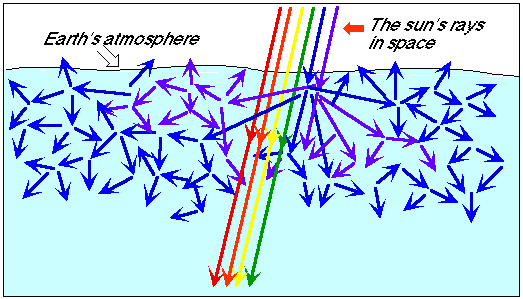
\includegraphics[width=0.5\textwidth]{Imagenes/rayleigh_scattering.png}
  \caption{Esquema del scattering de Rayleigh de la luz blanca en la estrat\'osfera}
  \label{fig:rayleigh_scattering}
\end{figure}

\paragraph{Suceptibilidad diel\'ectrica}
En la secci\'on siguiente hallamos la rigidez con que un electr\'on est\'a correspondido a un \'atomo o una mol\'ecula, y \'esto se puede medir en cantidades macrosc\'opicas a su vez por las fluctuaciones del campo el\'ectrico causado por una arreglo de \'atomos id\'enticos.\\
En esta secci\'on intentaremos formalizar el paso de las propiedades microsc\'opicas de una mol\'ecula, y las propiedades macrosc\'opicas del material que componen. Para simplicidad supongamos las moleculas son \textit{no polares} y lo suficientemente alejadas para que el campo que produzca una no sea influenciado por el de la otra.

\subparagraph{Campos constantes}
Supongamos un material dado se encuentra en un campo el\'ectrico constante de magnitud $E$, entonces va a inducir un campo de densidad de polarizaci\'on con magnitud $\mathcal{P}$ que en todo punto representa el momento dipolar por unidad de volumen. Entonces definimos:

\begin{equation}
\chi_e \equiv \frac{\mathcal{P}}{\epsilon_0 E}
\label{suceptibilidad_campocte}
\end{equation}

que llamaremos \textit{suceptibilidad el\'ectrica} de un material dado. Hay muchos efectos macrosc\'opicos que nos permiten medir $\chi_e$ aunque el m\'as simple es rellenar un capacitor (una disposici\'on de dos conductores con carga opuesta) y medir la nueva capacidad (la cantidad de carga que puede almacenar con una dada diferencia de potencial el\'ectrico) de \'este, que ser\'a la anterior aumentada en $1+\chi_e$.\\
Entonces si llamamos a $N$ como la densidad de electrones polarizables por el material por molecula por unidad de volumen, con una rigidez $k$, el desplazamiento producido por el campo $E$ ser\'a $eE / s$ dando un campo de polarizaci\'on:

\[\mathcal{P}=Ne^2 E / s\]

Dando una suceptibilidad:

\begin{equation}
\chi_e = \cfrac{N e^2}{\epsilon_0 s} = \left( \frac {\omega_p}{\omega_0} \right) ^2
\label{suceptibilidad}
\end{equation}

Que vale definiendo:

\begin{equation}
\omega_p^2 \equiv \left(e^2 / m_e \epsilon _0\right) N = (3,18 . 10^3 \ m^3s^{-2})N
\label{frecuencia_corte}
\end{equation}

Podemos recordar de \ref{frecuencia_plasma_simple} y vemos una similaridad con un $N$ definiendo la cantidad de electrones "en acci\'on" por unidad de volumen; con la diferencia que all\'i los electrones est\'an libres y aqu\'i est\'an retenidos al material.\\
Usando \ref{suceptibilidad} podemos obtener la frecuencia de resonancia a partir de $\chi_e$.

\subparagraph{Campos alternos}

En un campo alterno seguramente ser\'a funci\'on de la frecuencia $\chi_e(\omega)$. n general podr\'iamos adaptar \ref{suceptibilidad} a un campo alterno cambiando $1 / s$ por la compliancia $K(\omega)$ y tener, recordando \ref{frecuencia_corte}:

\begin{equation}
\begin{array}{rcl}
\chi_e (\omega) & = & m_e \omega_p ^2 K(\omega) \\
& = & \cfrac{\omega_p ^2}{\left(\omega_0 ^2 - \omega ^2\right) + i\gamma \omega}
\end{array}
\label{suceptibilidad_campoalt}
\end{equation}

Lo que produce a la suceptibilidad no solo dependiente de la frecuencia,sino tambi\'en compleja! Y esto nos indicar\'a que la polarizaci\'on esta atrasada al campo alterno, lo que nos indica claramente absorci\'on y entonces el material tender\'a a calentarse. Claramente estos efectos ser\'an observables en la zona de resonancia que cae en los $10^{15} Hz$ o m\'as y por esto veremos mucho mas de estos efectos en la segunda parte cuando tratemos con ondas que alcancen estas frecuencias, las electromagn\'eticas.

\paragraph{Absorci\'on de microondas por el agua}
El agua es un compuesto polar cuya formula es $H_2O$ (wooo,posta?) y que, por ende, presenta tres efectos capaces de contribuir a la polarizaci\'on total en el campo el\'ectrico circundante. El primero de estos es el cambio en el momento dipolar de los \textit{electrones} de la mol\'ecula, efecto que ya discutimos. El segundo corresponde al efecto de la vibraci\'on molecular de los \textit{\'atomos} con entre si, efecto que se puede visualizar en el infrarrojo (El que le gusta saber mas este efecto se explota en la identificaci\'on de mol\'eculas sobre todo org\'anicas en la espectroscopia de infrarrojo). Finalmente, la mol\'ecula \textit{como un todo} puede vibrar respecto a su centro de masa generado por torque oscilante del campo el\'ectrico. Dado que ninguno de estos efectos entonces puede explicar el aumento de la potencia absorbida del agua en la zona de microondas (se empieza a comportar como un \textbf{cuerpo negro}), vamos a analizar las \textit{rotaciones} de la mol\'ecula como efecto del torque del campo el\'ectrico que es un efecto que cae en las microondas. Para esto seguiremos los siguientes pasos 

\begin{enumerate}
\item Estimaremos la tension torsional $c$ que evita que el agua se alinee al campo el\'ectrico externo; lo que nos permitir\'a obtener un estimado de $\omega_0$
\item Estimaremos la resistencia angular $d$ de las fuerzas que evitan la rotaci\'on libre (an\'alogo a $b$ en el amortiguado lineal), lo que nos llevara a estimar $\gamma$ y llegar a la conclusi\'on que el sistema esta fuertemente amortiguado ($\gamma\gg\omega_0$)
\item Obtendremos v\'ia $c$ y $d$ el tiempo de relajaci\'on para observar que $\tau_r\omega_0>1 \Leftrightarrow \omega \gtrapprox 10^{10} Hz$ que es exactamente la zona de las microondas.
\end{enumerate}

\subparagraph*{Tensi\'on t\'ermica}
En la ausencia de un campo el\'ectrico externo, las mol\'eculas de agua toman direcci\'on al azar; pero al encender un campo hay una tendencia a alinear los momentos dipolares con el campo unilateralmente. No obstante, tenemos por otro lado la agitaci\'on t\'ermica (viejo enemigo si recordamos el plasma, que no os preocup\'eis ya volver\'a a aparecer!) que restaura el movimiento al azar. Entonces dado un campo $E$ y un momento dipolar $p$ a un angulo $\theta$ tenemos

\[\langle{E,p}\rangle=p_E=p\cos(\theta)\]

Por otro lado del electromagnetismo cl\'asico se obtiene

\begin{equation}
\langle{p_E}\rangle=\cfrac{p^2 E}{3kT}
\label{momento_dipolar_promedio_microondas}
\end{equation}

Con el valor de $p\approx 6,1.10^{30} C m$ (la del $H_2O$)a temperatura ambiente y un campo de $E=10^5 V m^{-1}$

\[\cfrac{p E}{3kT}\sim 10^{-4}\]

Supongamos entonces que las mol\'eculas de agua no interact\'uan unas con otras fuertemente, entonces para una mol\'ecula en un angulo $\theta$ sin un campo externo, al encender el campo este producir\'a un $\delta\theta$ con:

\[\delta\theta=\cfrac{pE\sin{\theta}}{c}\]

Donde $c$ es una tension imaginada por un cable que es el que produce la tension torsional y hallaremos c para que obtengamos un resultado como el experimental, luego con el momento de inercia ya tendremos el $\omega_0$

Entonces el encendido del cambio produce un cambio en la polarizaci\'on

\[
\begin{array}{rcccl}
p'_E & \equiv & \delta p_E & = & -\cfrac{d}{d\theta}\left(p\cos(\theta)\right)\delta\theta \\
& & & = & p \sin {\theta} \delta\theta \\
& & & = & p^2 \sin^2 {\theta} \cfrac{E}{c}
\end{array}
\]

Como empezamos con una distribuci\'on al azar de \'angulos $\theta$ entonces la distribuci\'on de $\theta$ es $\propto 2\pi \sin(\theta)d\theta$. Entonces:

\[
\begin{array}{rcccl}
\langle{p'_E}\rangle & = & \cfrac{\left(\cfrac{p^2 E}{c}\right)\int_{0}^{\pi}\sin^3{\theta} d\theta}{\int_{0}^{\pi}\sin^3{\theta} d\theta} & & \\
& = & \cfrac{\left(\cfrac{p^2 E}{c}\right)[\cfrac{1}{3}\cos^3{\theta}- \cos{\theta}]_{0}^{\pi}}{[\cos{\theta}]_{0}^{\pi}} & = & \cfrac{2 p^2 E}{3c}
\end{array}
\]

Como $\langle{p'_E}\rangle = \langle{p_E}\rangle$ de \ref{momento_dipolar_promedio_microondas} tenemos ya un valor de $c$ que corresponde a 

\[c=2kT\]

Entonces a temperatura ambiente $c\approx 8.10^{21} N m$. Ahora necesitamos el momento de inercia del agua para poder tener la frecuencia de resonancia pues $\omega_0 = \sqrt{\cfrac{c}{I}}$ (Aunque no lo pusimos de ejemplo el lector lo puede pensar como un engranaje oscilando libremente con un cable que le ejerce una fuerza de retorno $T_r \propto \psi$ con constante de proporcionalidad $c$). Si imaginamos al agua con el \'atomo de oxigeno central y dos pelotas representando los hidr\'ogenos, su momento de inercia sera

\[I\approx 2m_p R_{OH} ^2\]

que toma el valor de $I \approx 3,5 . 10^{-37} \ kg m^2$ y por ende $\omega_0 \sim 10^{13} \ s^{-1}$ es el valor de la frecuencia de resonancia

\textbf{Ejercicio:} Releer la demostraci\'on anterior hasta poder llegar a decir convincentemente que tiene sentido, cuando no lo logre recurra al libro, si lo logra, b\'usqueme a explic\'armela a mi. 

\subparagraph*{Una estimaci\'on de $\gamma$}
No se preocupen este viene mas corto y entendible jaja. El movimiento en general esta amortiguado porque cada mol\'ecula de agua rotante tiene un \textit{entorno} que arrastra al rotar y le va quitando energ\'ia intuitivamente, lo que tomamos por \textit{viscosidad} del fluido. Supongamos que nuestra mol\'ecula de agua es esf\'erica en un medio continuo viscoso, entonces queremos averiguar

\begin{equation}
T_r \equiv -d\dot{\psi}
\end{equation}

Tomando el an\'alogo de la fuerza amortiguante en \ref{eq:oscilador_amortiguado}. Como la fuerza $T_d$ ejerce un torque sobre la superficie esf\'erica, podemos estimar \[T_r= R F_r\] donde $R$ es el radio de la esfera(que en qu\'imica se le llama el \textbf{radio de Van der Walls} de la mol\'ecula) y $F_r$ representa un promedio de las fuerzas amortiguantes sobre la mol\'ecula. Si consideramos al fluido laminar y que desliza por la mol\'ecula, entonces la velocidad del fluido es de $a\dot{\psi}$ y podemos suponer que esta cae a 0 en una distancia $a$ dado que consideramos la interacci\'on \textit{solo} con las mol\'eculas rondantes. Por ende

\[F_d \approx - \left(4\pi a^2\right)\eta\dot{\psi}\]

pues debe ser proporcional a la viscosidad, al \'area de la esfera y a la velocidad promedio del fluido que, suponiendo la ca\'ida lineal que dijimos, representa a $\nabla \psi = \dot{\psi}$; esto nos lleva a 

\begin{equation}
d \approx 4 \pi \eta a^3
\end{equation}

Y usando los valores experimentales tenemos que $d\approx 9.10^{32} N m s$. Por lo que

\[\gamma \equiv \cfrac{d}{I} \sim 10^{15} \ s^{-1}\]

Con lo que juntando todo $Q \sim 0.01 \ll 1$ y por ende el amortiguamiento es muy fuerte.

\subparagraph*{El tiempo de relajaci\'on}
Para definir el tiempo de relajaci\'on en las vibraciones rotacionales podemos ver \ref{tiempo_de_relajacion} que es el factor de amortiguamiento sobre la constante de la fuerza de retorno, lo que lleva natural extenderlo a 

\[\tau_r = \cfrac{d}{c}\]

con lo que

\[\tau_r \approx \cfrac{2\pi\eta a^3}{kT}\]

que nos da un valor de $\tau_r \approx 10^{-11} \ s$ y por ende obtenemos que $\omega\tau_r \sim 1 \leftrightarrow \omega \gtrapprox 10^{11} \ s^{-1}$ que nos da una $v_0 \sim 10^{10} \ Hz$ que es la zona del microondas y por eso funciona el microondas! (woaaa, prefer\'ia no saber, no?)

\end{document}